The lunar farside provides a unique radio frequency (RF) environment in our Solar System in that the moon shields it from Earth and near-Earth RFI at all times. Therefore, {\em anything} detected there is of scientific interest. Since there is no ionospheric blockage, low-frequency observations that are impossible from Earth can also be made in this RFI-free environment.

Note that the science case contains science from a number of categories:
(1) science where LFT3 can do unique science that cannot be done or done as well from Earth;
(2) science where LFT3 provides useful additional information that could be used in addition to observations that can be done from Earth;
(3) science that demonstrates that LFT3 works and provides confidence in the performance of the telescope and lunar operations.  For guidance, the science case is {\em not} predicated on what might be done if one had a fairly large budget to design and build a radio telescope on Earth, but rather what could one do for an inexpensive lunar mission that advances science and our understanding of operating on the moon.

Although the lunar farside will remain an excellent low-RFI site for many years to come, {\em now} is the only time to take completely pristine measurements of the radio spectrum. This is an opportunity that will never again present itself, as seen in Fig. \ref{fig:missions}, with more than three dozen lunar orbiters planned before 2030.  This section discusses the primary science cases that drive the design of the array, which are summarized in the science traceability matrix in Appendix A.

\subsection{Technosignatures}
Humanity's quest to determine its place in the Universe and whether we are its only inhabitants has driven our imagination and quest for knowledge since we first looked to the sky.  Many large telescopes across the electromagnetic spectrum are being planned and developed to help determine if biological processes are happening around nearby stars (called ``biosignatures'').  We now also have the capability to explore whether technological signals (``technosignatures'') exist over a large swath of our Galaxy.  The Breakthrough Listen program \citep{2016iac..conf34378W} has transformed the field and has greatly expanded the search for such technosignatures (e.g. \citealt{Enriquez_2017, Price_2020, Gajjar_2021}).  The greatest technical impediment in this endeavor is the prevalence of RFI made by essentially every device on and around Earth that is electrically powered.

Although RFI is prevalent, excellent technosignature searches can be conducted from the Earth, particularly from remote locations where terrestrial interference is low and at frequencies that, at that time and place, are free of interfering signals. Excision techniques, as mentioned above, are generally used to flag RFI based on statistical methods and can be very effective.  However, it is noted that technosignatures, being of artificial origin, have characteristics similar to RFI and may be thrown out in this process, and that excision also represents an opportunity lost to making a detection.  The prevalence of RFI also renders any eventual detection less certain as any signal could be the result of pathological RFI.  The recent experience of Breakthrough Listen Candidate 1 highlights this \citep{2021NatAs...5.1153S}.

Figure \ref{fig:bubbles} provides a high-level summary of the coverage of ground-based radio searches, both ongoing and completed (circles). The purple and red-shaded regions show two of the large program ground-based technosignature searches currently in progress. For Earth-based searches, in order to further guard against interference, one usually uses a cadence of a series of on-target and off-target observations, where the ``off'' can be the ``on'' for another target. The use of this in a multibeam system like LFT3 is demonstrated in \cite{Huang_2023}. Using a multibeam system allows ``on'' and ``off'' to be simultaneous, making it even more efficient (i.e., \citealt{multibeam}). Also, note that a remote site does not provide shielding from satellites and airplanes. Techniques exist to subtract or decorrelate interference, but they are not perfect and it seems unlikely that a technosignature detection ``through'' RFI would be believed, even if not immediately rejected in a pipeline, as would likely be the case.




\begin{figure}
    \centering
    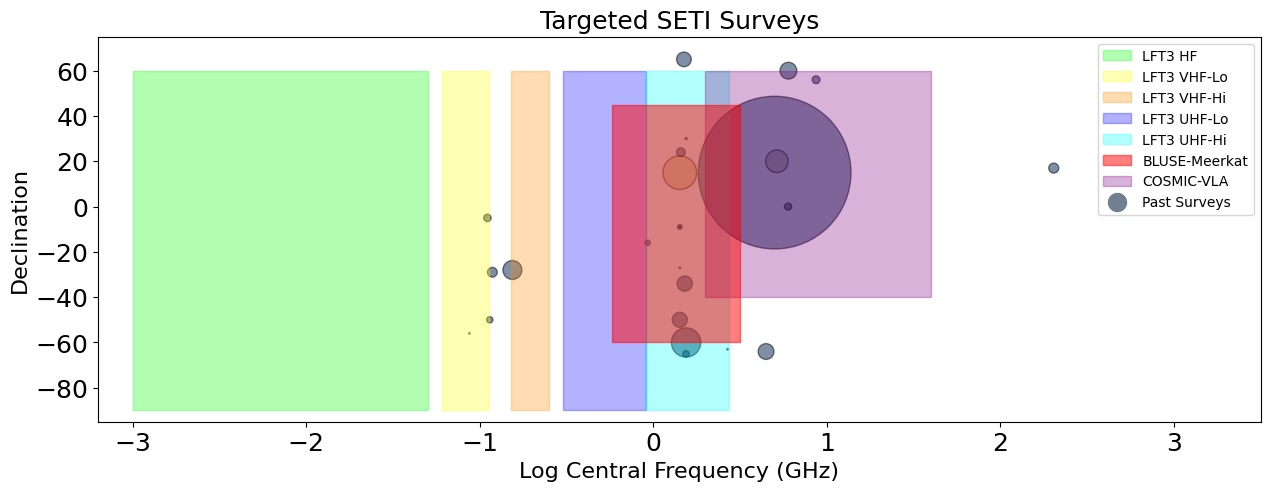
\includegraphics[width=0.85\linewidth]{figures/SETI_Bubble_LFT3.jpg}
    \caption{A plot of the historical technosignature searches (modified from \citealt{Tremblay_2022}). The circle size is scaled to the total number of targeted sources within the survey and located at the average declination. The colored rectangles show the regions in frequency and declination that LFT3 will cover as well as two large ground-based programs conducted by Breakthrough Listen and SETI Institute. As shown, LFT3 will survey regions that cover both new or rare regions (HF and VHF) as well as well-studied regions (UHF).}
    \label{fig:bubbles}
\end{figure}

Of course, we have no a priori information on any parameter of a technosignature, so one must search agnostically with the most sensitive receivers one can muster.  However, the initial signal detected will likely have a relatively high signal-to-noise ratio in some parameter space. For now, at radio wavelengths, that parameter space generally comprises frequency and time, and narrow-band or pulsed signals are the most likely to be detected.  They are also among the least likely signals to be confused with an astrophysical process \citep{Hippke_2017}, but are most likely to be confused with RFI. Within that parameter space, there is a case to be made that the most likely initial detection will be a slow transient arising from some underlying cadence such as a civilization targeting many distant worlds with a beacon or some fortuitous alignment such as the conjunction of two extrasolar planets with our telescope beam.  As mentioned in the Introduction, the ``Wow!'' signal is an exemplar of what one such signal could look like.  As also mentioned, if observed from Earth, even if that event occurred when it was not obscured by RFI, one would likely not have a high confidence of its origin due to the many sources of potential RFI. To reliably detect such a signal, one must go to a place where no other potential sources of emission reside.

In order to assess whether a small telescope can meaningfully search for technosignatures, it is instructive to look at detectability of various transmitter strengths for the stellar distribution around us. The Arecibo planetary radar (when it was operating) had been the highest effective isotropic power radiator at a level of greater than 20 TW and is a key fiducial. Another is to assume that an advanced civilization could produce significantly greater radiated power; in this case we will consider 1000 times that of the Arecibo planetary radar \citep{Gray_2020}.  Figure \ref{fig:isaacsonetal} shows the signal-to-noise ratios if hypothetical transmitters of this power were located near the stars in various star catalogs.  The black background catalog is the Breakthrough Listen target selection \citep{2017PASP..129e4501I} plus the stars within 100 light years (the black histogram is the total and the colors break down by stellar type) and the gray background (bottom only) is for stars from the Gaia Nearby Stars Catalogue \citep{2021A&A...649A...6G}. As shown, even {\em our} current technology provides a detectable signal to this telescope, let alone a stronger signal from a more advanced civilization.

\begin{figure}
    \centering
    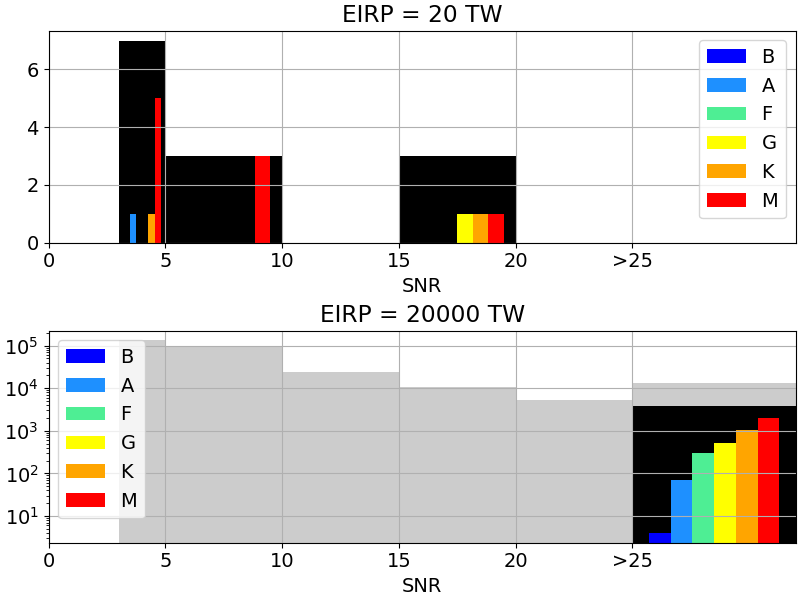
\includegraphics[width=0.75\linewidth]{figures/catcounts.png}
    \caption{LFT3 detection sigal-to-noise ratios (SNR) for the Breakthrough Listen target selection \citep{2017PASP..129e4501I} and a catalog of stars within 100 light years (https://chview.nova.org/solcom) for an ``Arecibo'' scale transmitter (top) and 1000 times larger (bottom).  The black background is the total number per SNR bin and the colors are the individual spectral types.  The first bin extends from 3-5 and the last bin is 25 and greater.  The light gray on the bottom plot shows the same calculation for all of the stars in the Gaia Nearby Star Catalogue \citep{2021A&A...649A...6G} along with the other catalogs.}
    \label{fig:isaacsonetal}
\end{figure}

% Paragraph below is now redundant.
% Signals of interest must be carefully sought within this cacophony of RFI. To differentiate between RFI and a technosignature requires that the technosignature signal is at a frequency/time not inhabited by RFI and the signal must persist and be quite stable over a timeframe of many minutes.  The signals are assumed to be nearly monochromatic and slow-drifting in time.  A series of on-off measurements are used (for single-dish experiments)to make sure that the signal-of-interest is coming from the main beam of the telescope and not RFI in a distant sidelobe.  These techniques are incredibly powerful in conducting senstive searches over the available bandwidth, and have the added benefit being able to use very large earth-based telescopes to dramatically increase the sensitivity.  However, many limitations exist on appropriate ranges of frequency and time, and some frequency ranges are so impacted that searches (and radioastronomy research generally) are infeasible in those bands.  Signals of short duration (a few seconds) or signals heavily modulated are nearly impossible to discern.  And of course, technosignatures ``behind'' RFI is not detectable (or at least believably so).

%With online beamforming capabilities we can search the nearest stars  across a range of frequencies rarely searched from Earth but represent some of our most power transmitters \citep{Tremblay_2022}. Within the current FPGA framework, calibration and dynamic spectrum creation can be completed giving us access to the full details of the signals detected for each frequency range. This combined with a sample of the time-averaged spectrum will provide a unique dataset in which to seek an answer to ``Are we alone?". Assuming a civilization is capable of building a big dish to generate an isotropically distributed signal of $\sim$10${^17}$\,W, with a 6$\sigma$ sensivity of 0.5\,Jy, we could expect to detect that signal out to about 3\,pc. However, a beamed signal or a large megastructure is expected to create power over 10$^{26}$\,W. 

%The $Gaia$ Space telescope has given has a large catalog of targets which we are already using in blind, commensal surveys with MeerKAT (Czech et al. in prep) and the Karl G. Jansky Very Large Array \citep{Tremblay_2024}. From this experience we can develop and efficient search working on the FPGA framework.

\textbf{System Implications:} As shown in Figure \ref{fig:bubbles}, the proposed telescope frequency covers a new parameter space in technosignature searches, especially with HF and VHF receivers. Technosignatures are likely to emit into a single polarization state and therefore polarization sensitivity is needed. The technosignature science case requires some in-line processing of the data to find signals of interest and generation of dynamic spectra or raw voltage postage stamps around signals of interest. In the commensal system, real-time is used in MeerKAT \citep{Czech_2021} and VLA \citep{Tremblay_2024}, \textsc{seticore} \footnote{\url{https://github.com/lacker/seticore}} to search for signals toward beam-formed targets. \textsc{seticore} uses an efficient Taylor-Tree de-dispersion algorithm to autonomously search for narrowband signals. The user specifies the signal-to-noise ratio to identify signals of significance and the drift-rate search width. To save on information needing to be transferred to the ground, one could de-disperse the signal and only transmit the time averaged power spectrum instead of sending the entire dynamic spectrum. As there is no known technosignature signal thus far identified, frequency resolution and time resolution are open parameters that are flexible to the needs to keep data rates and processing to a minimum.  Section \ref{sec:conops} will outline the concept of operations given the highly constrained mission parameters.  The nominal specifications are 1 sec time resolution and 10 Hz frequency resolution.

We can verify these modes of operation by looking toward Mars, where there are a number of space-based and ground-based communication signals transmitted back to Earth on a regular basis, as well as for lunar orbiters. The carrier signals are typically emitted at 2200-2290 MHz and represent a population of narrow-band artificial signals.
The sky rotates $\approx$ 30 times slower when observing from the Moon's surface compared to Earth. This allows longer dwell times on a given patch of sky, which in turn allows prolonged studies of signal characteristics. 

\subsection{Transients}
In the last 20 years, the field of radio transients (both slow and fast) has brought a wealth of information, significantly advancing various areas of physics. In particular, pulsars and fast radio bursts (FRBs) stand out because of their unique potential to reveal new types of physics \citep{beskin_radio_2015, ng_brief_2023} and understanding of the fabric of spacetime. These astrophysical phenomena offer valuable insight into gravitational waves, cosmology, and plasma physics, among other fields. However, radio observations can also shed light on other transients, such as flare stars and planetary conditions within the Solar System. Overall, the strength of a lunar-based telescope is in discovering the unknown. This includes the possible detection of various `low-DM' (or dispersion measure, an indicator of relative proximity) events, on timescales of milliseconds to minutes.  Such events may include low-DM FRB analogues, FRBs from Galactic magnetars, decimetric solar bursts, stellar bursts, and undiscovered time-domain phenomena. In particular, LFT3 would uniquely enable the discovery of new populations of transient astrophysical sources in the very local Universe at 0--30~MHz and 87--108~MHz. Figure \ref{fig:transient_space} details various observational setups of LFT3 against well-known transients in the $\nu \text{W}$ vs $L_\nu$ parameter space along with minimum detectable flux density values at various pulse widths.
%detailed in table \ref{tab:smin}.

\begin{figure}[!ht]
    \centering
    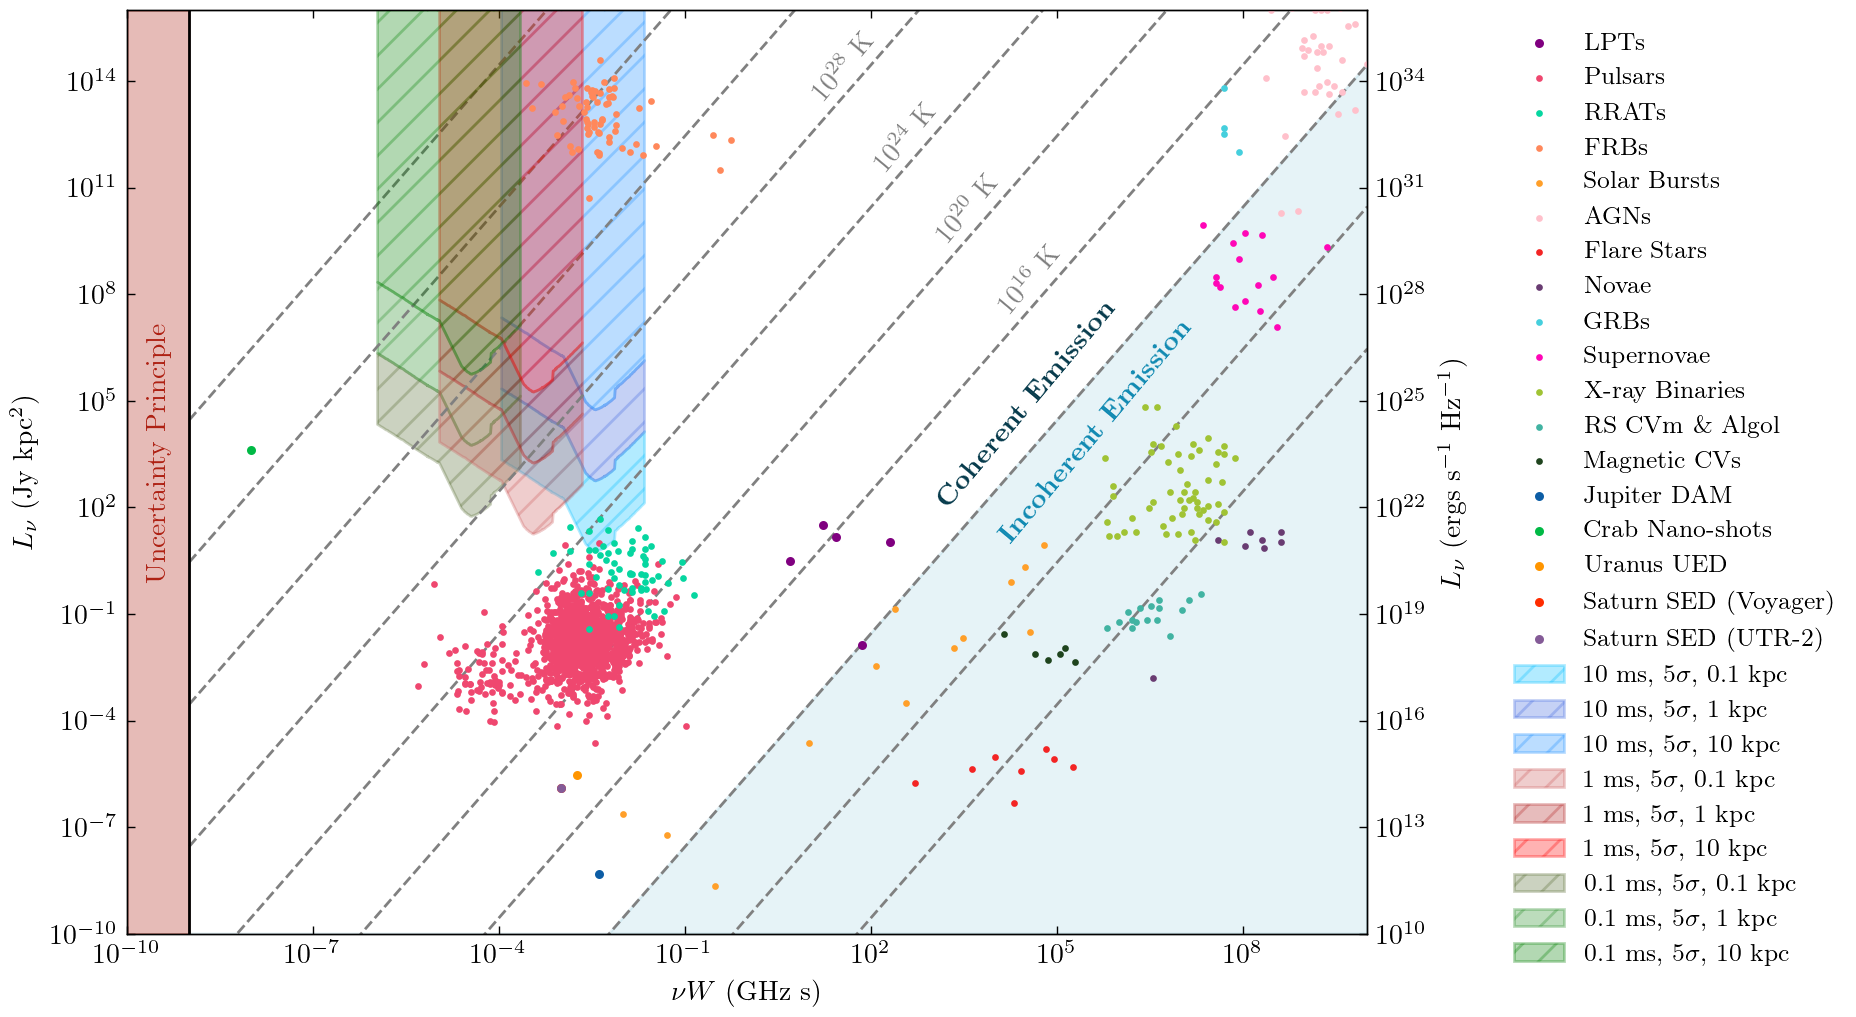
\includegraphics[width=0.9\textwidth]{figures/phase_space.png} 
    \caption{Transient Parameter Space figure adapted from \citet{pietka}. This plot illustrates the sensitivity regions of a LFT3 observational setup across different pulse widths (0.1~ms, 1~ms and 10~ms) at 1~kpc on a $\nu \text{W}$ vs. $L_\nu$ phase diagram. Where $\nu \text{W}$ represents the product of observed frequency and pulse width and $L_\nu$ shows the spectral luminosity. The blue, green and red hashed regions correspond to a pulse width and show the detectable signal levels above a threshold of $5\sigma$ for the LFT3 bandwidth.}
    \label{fig:transient_space}
\end{figure}





% Emission from planets has also been observed in the form of auroral emission. The most notable example of this is the Jovian system. The Jovian system is known to have auroral emission that is driven by the interaction of the solar wind with the magnetosphere of the planet. Coherent radio emission from the aurora is thought to be produced through the cyclotron maser instability \citep[ECM;][]{zarka_auroral_1998} which injects a high-velocity electron population into the magnetosphere. The maximum frequency of the ECM is directly proportional to the magnetic field strength of the object at its emitting point \citep{kavanagh_hunting_2023, joe_nature_review}.


\subsubsection{Solar Physics}
Low-frequency studies of the Sun date back to the early days of radio astronomy, with some of the first published observations appearing in 1963~\citep{Wild_1963}. Despite this early start, a new generation of instruments, including LOFAR and the MWA, has enabled significant advances due to wider bandwidths, improved telescope design, and enhanced computational capabilities. Key science goals include the study of non-thermal emissions, gyrosynchrotron emission associated with coronal mass ejections (CMEs), targeted analyses of solar bursts (Types I--V), and polarimetric measurements. Many of these studies require high-bandwidth imaging on short time scales~\citep{Kansabanik_2022}, though the spectral-temporal characteristics of quiescent versus active solar states are also of interest given their impact on Earth-based technologies.

One of the significant outstanding questions in heliophysics is: ``How does the Sun produce strong southward-pointing magnetic fields in solar CMEs that lead to geomagnetic storms, and can such storms be predicted?'' In an effort to explore the connection between CMEs and phenomena such as Type II bursts, solar flares, and shocks, \citet{Bastian_2001} analyzed observations at 150 and 450\,MHz with 32\,s integration and $\sim$1\,MHz spectral resolution. Their work yielded constraints on thermal plasma density, density filling factors, relativistic electron number density, and magnetic field strength within CMEs -- values still widely referenced today.

Solar observations at varying time and frequency resolutions remain challenging. A farside lunar telescope would offer a dynamic spectral view of solar activity across a frequency range unobservable from Earth and not explored in detail since the Voyager missions of the 1970s. As the Sun approaches solar maximum, such a telescope would be uniquely suited for capturing transient low-frequency events, such as Type II/III bursts and solar-driven auroral emissions from planetary bodies. 

Interplanetary scintillation (IPS) observations from the lunar farside could be used to pinpoint solar wind and heliophysical structures by measuring the rapid intensity fluctuations of the compact radio background caused by turbulence in density regularities in the solar wind \citep{fallows_application_2023}. This technique could potentially reveal bulk flow velocities and turbulence levels and detect large-scale heliospheric density structures (e.g., tracking CME-driven shocks) throughout the inner heliosphere. Compared to Earth-based IPS experiments \footnote{e.g., with the MWA and LOFAR operating at $80$–$300~\text{MHz}$, \cite{fallows_separating_2016} and \cite{kaplan_murchison_2015}} that are limited by terrestrial ionospheric distortion, LFT3 could lend its low observing frequency phased array to achieve higher angular resolution \citep{DEX}. 

% \textbf{System Implications:} High-time-resolution dynamic spectra ($\sim$1--2\,ms) with $\leq$0.5\,MHz spectral resolution would significantly benefit the solar physics community. Coordinated observations with other low-frequency instruments, such as the MWA or LOFAR, would provide coverage over a broader spectral range. Such data products would be valuable during both active and quiescent solar phases. The inclusion of Stokes V dynamic spectra at comparable resolution would offer additional diagnostic capability.

\textbf{System Implications:} High-time-resolution dynamic spectra with time resolution on the order of 1--2\,ms and spectral resolution of $\leq$0.5\,MHz would be critical for resolving fast-evolving solar radio bursts, particularly Type III. Coherent bursts from solar events can reach flux densities of $\sim$10$^3$--10$^6$~Jy, but occur over narrow frequency bands and short durations, requiring fine temporal and spectral sampling for full characterization. Dynamic spectra in both Stokes parameters I and V would allow for polarimetric studies of coronal magnetic fields and emission mechanisms. Low-frequency IPS studies require long integration baselines (e.g., 10--100\,s) across a wide field of view to track scintillation patterns and infer bulk solar wind properties and density turbulence. \

The frequency range of interest spans $\sim$0.1--30\,MHz, encompassing the decametric and hectometric bands relevant for Type II/III solar bursts and the IPS regime. This range lies entirely below Earth's ionospheric cutoff, making space deployment essential. A phased array configuration with beam steering would facilitate flexible observation of both targeted and wide-field events. Coordinated observations with MWA, LOFAR, and space-based platforms like SunRISE would enable multi-instrument solar diagnostics across a broader frequency range and heliocentric baselines. These data products would be valuable across both active and quiescent solar phases, contributing to long-term solar monitoring and forecasting of geomagnetic activity. 


%\textbf{Calvin: no mention of LWA? I would be surprised if they didn't do some kind of solar monitoring! More broadly, it's unclear what LFT3 adds here to a reader who is unfamiliar with interplanetary scintillation techniques (disclaimer: I am a big fan of IPS). Also, it's not clear that you can't do the proposed science from a telescope above the ionosphere, which isn't that high.}


\subsubsection{Solar System Emission} 
There exist numerous sources of radio emission throughout the solar system. Most notably, Jupiter's strong magnetic field interacts with its moons, particularly Io~\citep{Io}, but also Europa and Ganymede~\citep{Corentin}, producing intense MJy-level auroral radio emissions. Jupiter emits over a broad frequency range from 10~kHz to 40~MHz~\citep{zarka_auroral_1998}, with its hectometer-wavelength (1--5~MHz) emission modulated by solar wind activity~\citep{Desch1984}. The electron cyclotron maser instability~\citep[ECMI;][]{EMI}, a plasma instability that occurs in magnetized environments with energetic electron populations, is the main driver of the Jupiter emission \citep{zarka_auroral_1998}. Jupiter is the only planet in the solar system\footnote{Auroral radio emissions from Earth, Saturn, Uranus, and Neptune have all been detected but the observed frequencies are all below 1 MHz \citep{zarka_auroral_1998}.} whose ECMI radio emission can be seen from the ground due to the ionsphsheric cuttoff \citep{zarka_auroral_1998}. A lunar-based telescope would enable observations of these low-frequency bands, particularly around solar maximum, offering an opportunity to study solar-wind-driven dynamics in the Jovian system. This study can also be used as a benchmark for studying exoplanet radio emission from close-in exoplanets \citep{Zarka2007,joe_nature_review}. 

%The electron cyclotron maser instability~\citep[ECMI;][]{EMI}, a plasma instability occurring in magnetized environments with energetic electron populations, is thought to be a key emission mechanism in both solar and stellar contexts. ECMI is considered to be the primary driver of coherent radio emission observed on Jupiter, where electron beams accelerated in the corona generate strong, polarized emission. Understanding the conditions that trigger ECMI and the characteristics of the resulting emission is essential to studying solar radio physics at low frequencies.

%A lunar telescope is also well-suited to probe low-frequency emission from the other planets of the outer Solar System.  During its flyby, \textit{Voyager 2} detected strong $\sim$100~Jy radio emissions from both Uranus and Neptune, indicative of the presence of strong planetary magnetic fields \citep{zarka_auroral_1998, ZHANG199237}. One high-priority science case is the re-detection of these emissions from these planets 

A lunar telescope is also well suited to probe low-frequency emission generated by lightning from the solar system. In particular, LFT3 can study the radio emissions generated by lightning from Venus, Mars, Saturn, Uranus, and Neptune. Radio detections of lightning have been found on Uranus from 900 KHz--40~MHz using Voyager \citep{1986Zarka_Emission} and on Saturn from 2--30~MHz using Voyager, Cassini, and UTR-2 \citep{Zarka2004}. Tenative detections of Neptune lightning from 20-30 MHz were observed by Voyager 2 \citep{Kaiser1991}, but they remain unconfirmed. Lightning radio emissions from Venus (2- 30 MHz) and Mars (20-30 MHz) are also predicted to occur, but have not been observed \citep{Zarka2008}. Despite subsequent attempts using LOFAR and NenuFAR, the emissions from Saturn and Uranus have not been detected again, likely due to Earth's ionosphere and low-cadence observations. Likewise, searches for lightning on all the solar system planets are ongoing at NenuFAR. LFT3 is unqiue as it would allow for a relatively long-term observing campaign with no RFI. A confirmed re-detection or new discovery would carry significant implications for understanding planetary atmospheres, magnetospheres, and the general nature of the weather on planets in the outer Solar System. 

%Voyager's low-band instrument also observed emissions associated with lightning activity (900 KHz--40~MHz) on Uranus~\citep{1986Zarka_Emission}. Saturn's lightning-induced radio emissions, which span from 2 to 30~MHz and reach intensities of $\sim$1000~Jy, present another valuable target for low-frequency monitoring~\citep{Zarka2004}.


\textbf{System Implications:} Dynamic spectra in Stokes parameters I and V with high time resolution (e.g., subsecond to a few seconds) would enable the characterization of emission morphology and polarization. Known radio flux densities from outer Solar System planets span a wide range, from $\sim$100~Jy (Uranus lightning; \citealt{1986Zarka_Emission}) to $\sim$1000~Jy (Saturn lightning; \citealt{Zarka2004}), and up to MJy levels for Jupiter~\citep{zarka_auroral_1998,ZHANG199237,Zarka2004}. Emission is typically concentrated between 0.1–40~MHz, a range that lies mainly below the Earth's ionospheric cutoff. The emissions associated with lightning are expected to have burst durations of seconds to minutes~\citep{1986Zarka_Emission}, requiring longer integration times and high spectral resolution (e.g., $\leq$100~kHz). A bandwidth covering at least 0.1–30~MHz is necessary to capture the full spectral envelope of lightning radio emissions. Additionally, dual-polarization capability is critical for distinguishing between thermal and non-thermal processes and identifying strongly polarized bursts.

\subsubsection{Exoplanet auroral radio emission} 
Exoplanets with and without a magnetic field are expected to behave and evolve very differently. Therefore, there is great need to directly constrain these fields to holistically understand the properties of exoplanets. To begin with, knowledge of a planetary magnetic field can provide robust constraints on the interior structure of a planet, including its composition and thermal processes \citep{G2015,Brain2024}. Historically, initial insights into the interior structure of the Solar System's gas giants were derived from the understanding that they possess magnetic fields \citep{Hubbard1973}. Furthermore, planetary magnetic fields will also affect (either enhancing or suppressing) atmospheric escape \citep{G2015,Zarka2018haex,Lazio2019,Egan2019,Brain2024}, atmospheric dynamics and evolution \citep{Perna2010a,Beltz2023}, and planetary formation \citep{Lovelace2008,Batygin2018,Jia2023}. Ohmic dissipation could also be one of the main factors contributing to the anomalously large radii of hot Jupiters \citep{Perna2010a,Batygin2010,Thorngren2018}, one of the longest-standing mysteries in exoplanet science. Finally, magnetic fields could potentially play a crucial role in sustaining the habitability of Earth-like exoplanets by providing protection against cosmic rays \citep{Gr2015,exss2018,Shahar2019} and aiding in understanding atmospheric escape mechanisms \citep{Lazio2019,Zarka2018haex,Kopparapu2020}. Likewise, studying terrestrial magnetic fields can offer insight into other aspects of the planet that could influence its habitability, such as the presence of tectonic plates or the size of the core \citep{Shahar2019,Kopparapu2020}.

Despite decades of effort, the direct detection of magnetic fields on exoplanets has remained elusive \citep{G2015,Brain2024}. There are many methods proposed to constrain the magnetic fields of exoplanets. Auroral radio observations, analogous to auroral radio emissions by solar system planets, are among the best methods to detect exoplanetary magnetic fields \citep{Zarka2007,Zarka2015SKA,G2015,Brain2024}, as many of the other methods are prone to false positives \citep{G2015,Turner2016a,Route2019}. This radio emission is predicted to be entirely driven by the stellar wind \citep{Zarka2007}. Therefore, the radio flux densities of exoplanets in close-in orbits are predicted to be orders of magnitude higher than Jupiter's radio flux density \citep{Griessmeier2007_AA,Griessmeier17PREVIII} and thus potentially detectable with modern low-frequency radio telescopes \citep{Zarka2015SKA,Griessmeier17PREVIII,Turner2019}. Recently, the first possible detection of an exoplanet, the hot Jupiter $\tau$~Boo~b, in the radio was reported from LOFAR \citep{Turner2021_Radio}. Follow-up radio observations are underway to confirm this detection of $\tau$~Boo~b are underway \citep{Turner2023_PRE,Turner2024}. Also, new observations from NenuFAR have found tentative hints of emission from another hot Jupiter system, HD 189733 \citep{Zhang2025}. A large-scale exoplanet survey with NenuFAR is currently ongoing. However, mainly close-in hot Jupiters can be studied from the ground due to the ionsphsheric cuttoff. 

The search for exoplanets with LFT3 would be unique and would greatly benefit the field. To start with, there has never been an exoplanet radio search between 1-10 MHz (with the exception of the upcoming LuSEE-Night mission with which LFT3 has the opportunity to collaborate). Likewise, the planets that can be studied in this frequency range are smaller than Jupiter and thus cannot be studied from the ground. Although individual bursts from an exoplanet cannot be seen with LFT3, several key aspects of the emission will allow for stacking of observations. Exoplanetary radio emission occurs over long time scales (minutes to hours) and large bandwidths (10s of MHz), and the emission is periodic (for tidally locked planets the emission beam will be pointed towards the observer during the same part of the orbit) and circularly polarized \citep{Zarka2007}. Therefore, we would be able to stack the entire dataset together to search for these exoplanet signals. This could be done by using a Lomb–Scargle periodogram, as recently verified on Jupiter observations from NenuFAR \citep{Louis2025}, or similar techniques. For close-in hot exoplanets, we can observe $\sim$50-100 orbits over the length of the nominal mission. Studying the radio-loud exoplanets found by NenuFAR and LOFAR (e.g. $\tau$~Boo, HD 189733) would allow us to verify this technique and enable the exploration of the outer parts of the magnetosphere that are not accessible from the ground. This study would place important constraints on the dynamo modeling, since this parameter space has never been explored before. Regardless of any detections, the science and technology lessons learned from LFT3 will help us better plan for larger radio telescopes (e.g., FARSIDE; \citealt{Burns2021_RSPTA}) on the Moon going forward.

\textbf{System Implications:} The exoplanet auroral emission is predicted to peak in LFT3's Low-band (1-10 MHz) for a handful of nearby exoplanets (Mauduit et al. in prep, Quentin et al. in prep). As the emission is predicted to be highly circularly polarized, only Stokes-V is needed. Previous detections from the $\tau$~Boo and HD 189733 systems range from 100's mJy to $\sim$2 Jy for individual bursts \citep{Turner2023_PRE,Zhang2025}. Flux predictions for some planets in the 1-10 MHz frequency range extend to $\sim$100 Jy for individual bursts (Mauduit et al. in prep, Quentin et al. in prep)\footnote{These studies are currently under embargo until published in Q3 2025.}. Therefore, exoplanets may only be obsevable only by binning over large time-scales ($\sim$10s hours) and large bandwidths ($\sim$10s of MHz) and searching through the entire dataset together. We would benefit from combining observations from LuSEE-Night together with LFT3, as the combined dataset would greatly increase the number of orbits. However, care must be taken when combining the two datasets, as the exoplanets may be experiencing very different stellar wind conditions between the observations. LFT3's low-band observations are complementary to ongoing ground-based searches, as LFT3 will probe different planet types. 

\subsubsection{Flare Stars}
Radio flare stars, which are often young, magnetically active stars, provide insight into stellar magnetic activity, star formation, and the early stages of stellar evolution. Observations from a farside lunar telescope could reveal details about the mechanisms driving these flares and their impact on the surrounding stellar environment. Studying radio flare stars also has implications for exoplanetary science, as the intense radiation from these flares can affect the habitability of orbiting exoplanets. Flare stars can also be used as a means of studying star-exoplanet interactions \citep{joe_nature_review}. A farside lunar telescope lends itself to assess the radiation environment of these planets, contributing to our understanding of exoplanet habitability based on the low frequency window observed and the unique lack of RFI there.

Observing these stars, especially at low frequencies ($\leq 300$ MHz), allows us to probe stellar and planetary plasma environments. Coronal Mass Ejections (CMEs) have a low-frequency burst component in which information about the kinematics of plasma can be deduced \citep{villadsen_ultra-wideband_2019}. The incident solar wind is also the primary driving force of auroral emission on magnetized planets. Radio emission from stars is typically produced through CMEs, observed phenomenologically in the Sun as type II and III solar bursts. They are also very radio-loud stars like CR Draconis peaking at 200~mJy at low frequencies \citep{callingham_low-frequency_2021} making their detection a viable science goal of LFT3. 

Much time has been spent observing Ultracool Dwarfs (UCDs, spectral type M7), as they provide a good analogue to the Jovian system. This provides valuable insights into the formation and atmospheric processes of both systems. Moreover, such comparative studies contribute significantly to understanding planetary evolution and diversity beyond our immediate neighborhood. Recent detection of radiation belts around a UCD further supports the analogy to Jupiter, since radiation belts are a key characteristic of Jupiter's magnetosphere \citep{joe_nature_review}. UCDs, being intermediate in mass between stars and planets, serve as a bridge to understanding exoplanet detection. The discovery of bursting radio emission from a brown dwarf and subsequent detections in UCDs indicate departures from established stellar coronal/flaring relationships. Radio bursts from UCDs can exhibit periodic timing \citep{hallinan_rotational_2006} along with strong circular polarization and high brightness temperatures, suggesting the involvement of the ECM process in generating radio emission. Despite a significant amount of gigahertz-frequency radio searches, the detection rates for UCD radio emissions remain stubbornly low at around 10\% overall at higher frequencies \citep{lynch_radio_2016}. Given that LFT3 will observe unique frequencies below 300 MHz, it can constrain the magnetic field strengths near the emission region of UCDs, offering significant insight into field geometry and strength not accessible at higher GHz frequencies.

It has also been suggested that exoplanetary magnetic fields can be studied using magnetic star-planet interactions (SPI) in the form of planet-induced radio emission \citep{Cuntz2000,Lanza2009,joe_nature_review}. Some hints are starting to emerge about SPI radio emission. This type of behavior has been confirmed between two magnetized stars in the T Tauri binary DQ Tau using radio bursts \citep{Salter2008}. Recently, \citep{Ilin2022,Ilin2024} examined both \textit{TESS} and \textit{Kepler} data of all exoplanetary systems and found hints of a tentative correlation between flares of the star and its hot Jupiter HIP 67522 b. HIP 67522 is also detected in the radio at GHz frequencies. In the radio, coherent radio bursts on the M dwarf YZ Ceti, which hosts a compact system of terrestrial planets, were observed from 2--4 GHz on the \textit{VLA} \citep{Pineda2023} and 550--900 MHz with the \textit{uGMRT} \citep{Trigilio2023}. Confirmation is still needed. These observations hint at an enhancement of detected bursts at specific orbital phases of the innermost Earth-like planet, YZ Ceti b, and modeling suggests that the magnetic field of the planet could be constrained with these observations \citep{Pineda2023,Trigilio2023}. A large-scale survey may find new SPI radio emission from nearby planet-hosting stars. The medium and high bands will be useful to search for star-planet interactions. 

\textbf{System Implications:} As mentioned, flare stars are radio-loud on the scale of tens of mJy at lower frequencies \citep{driessen_sydney_2024}. This puts nearby flare stars well within the realms of detection. As in the other science cases, LFT3 allows observations in previously contaminated or unreachable frequencies, with the FM and sub 30~MHz bands being of particular interest for monitoring already known bright sources \citep{joe_nature_review}. Time resolution of $\leq$100\,ms and spectral resolution of $\sim$0.1--0.5\,MHz would enable the detection and classification of coherent bursts, including ECMI-driven emission. Dual-polarization capability will be important to detect and analyze strongly circularly polarized bursts, which are diagnostic of magnetic field geometry and strength in stellar objects. 


\subsubsection{Pulsars}
Pulsars are highly magnetized rotating neutron stars that emit beams of electromagnetic radiation from their poles, analogous to the rotating light of a lighthouse~\citep{pulsar_handbook}. Pulsars serve as precise cosmic clocks, providing insight into the solar wind, interstellar medium, gravitational waves, and the fundamental physics of matter under extreme conditions \citep{sct+24,epta_inpta,ppta,agazie_nanograv_2023,Basu2025_SKA_EOS}. Pulsars are theorized to spin rapidly when they are created, but their rotation slows over time due to the combined braking effects of electromagnetic radiation, pulsar wind, and possibly gravitational wave emission~\citep{agf+16}. Using coherent dynamic spectra, sensitivity to weak pulses can be improved and frequency and time resolution can be adjusted to decrease the effects of dispersion measure smearing~\citep{cm03}. Figure \ref{fig:transient_space} shows the \textit{average} radio pseudo-luminosity values for the pulsar population; individual pulses can, however, extend several orders of magnitude higher \citep{karuppusamy_giant_2010}. LFT3 will perform single-pulse searches in order to detect the brightest subset of pulses. 


Broadband studies of pulsars allow for a study of their emission physics and surrounding material, where the lower frequencies are sensitive to emission closer to the pulsar surface \citep{hassall_wide-band_2012}. With ground-based radio telescopes, the ionosphere creates challenges, especially in weaker pulsars and those that have a spectral turn-over between 100--200~MHz \citep{Stappers_2011,jankowski_spectral_2018}. By moving the radio telescope off Earth, circumventing the ionospheric cut-off, which is typically around 30~MHz but can be higher, a new window of study for pulsar emission physics is opened. One of the lowest-frequency pulsar detections made to date has been with the Low Frequency Array~\citep{lofar} detecting emission down to 15~MHz with favorable ionospheric conditions \citep{Kondratiev_2013}.

%LFT3 could be well placed to observe some of the brightest pulsars below 15~MHz. 

%A farside lunar telescope, shielded from Earth’s RFI, would significantly enhance pulsar observations by providing a pristine observational environment. This location allows for low-frequency studies, critical for understanding the early stages of pulsar emission mechanisms and the surrounding interstellar medium. Furthermore, the lunar far side offers an opportunity to continuously monitor pulsars without interruptions caused by Earth's rotation, increasing data quality and allowing detection of subtle changes in pulsar behavior over time \citep{jankowski_spectral_2018}. 
% \textbf{CL: I love pulsars but I'm less compelled by LFT3 than by a pair of giant aperture arrays in Greenland and the South Pole, which are the two locations on Earth that don't have the cadence issue. The RFI rejection for pulsars is especially unimportant because the signal is periodic. I wish I had something more constructive here, but I don't know who the target audience is and what they might care about...let me know if you want to chat to brainstorm.}


\textbf{System Implications:} Beamformed data products are highly valuable for discovering a wide range of transient events, with pulsars being one of the potential beneficiaries.  LFT3 will provide extensive sky coverage, especially at lower frequencies; however, this comes with a reduced effective area (\(A_{\text{eff}}\)) and an increased sky temperature (\(T_{\text{sky}}\)), which lowers the overall sensitivity. Consequently, the pulsar candidates identified by LFT3 will likely be giant pulses; this is due to the luminosity distribution and pulse amplitude distributions of the Galactic pulsar population~\citep{bjb+12,k13,lbb+13,zgw+24,dwl+25}. %However, the ability to observe pulsar emissions in a pristine environment across a large bandwidth holds significant scientific value on its own. 
For some pulsars, with narrow pulse amplitude distributions, a periodicity-based search could yield detections based on the average flux densities. In Figure \ref{fig:pulsarDectability} we show the distribution of known pulsars potentially detectable by LFT3 with 10-hour coherently combined integrations, assuming flux densities reported in the ATNF Pulsar Catalogue~\citep{psrcat}.
% NB these are only 5sigma detections
% Might be good to give the 10sigma number
%LFT3 can be compared to instruments like Galactic Radio Explorer \citep[GREX;][]{GREX} which is designed to detect FRBs and Magnetar Bursts. 


\begin{figure}[h]
    \centering
    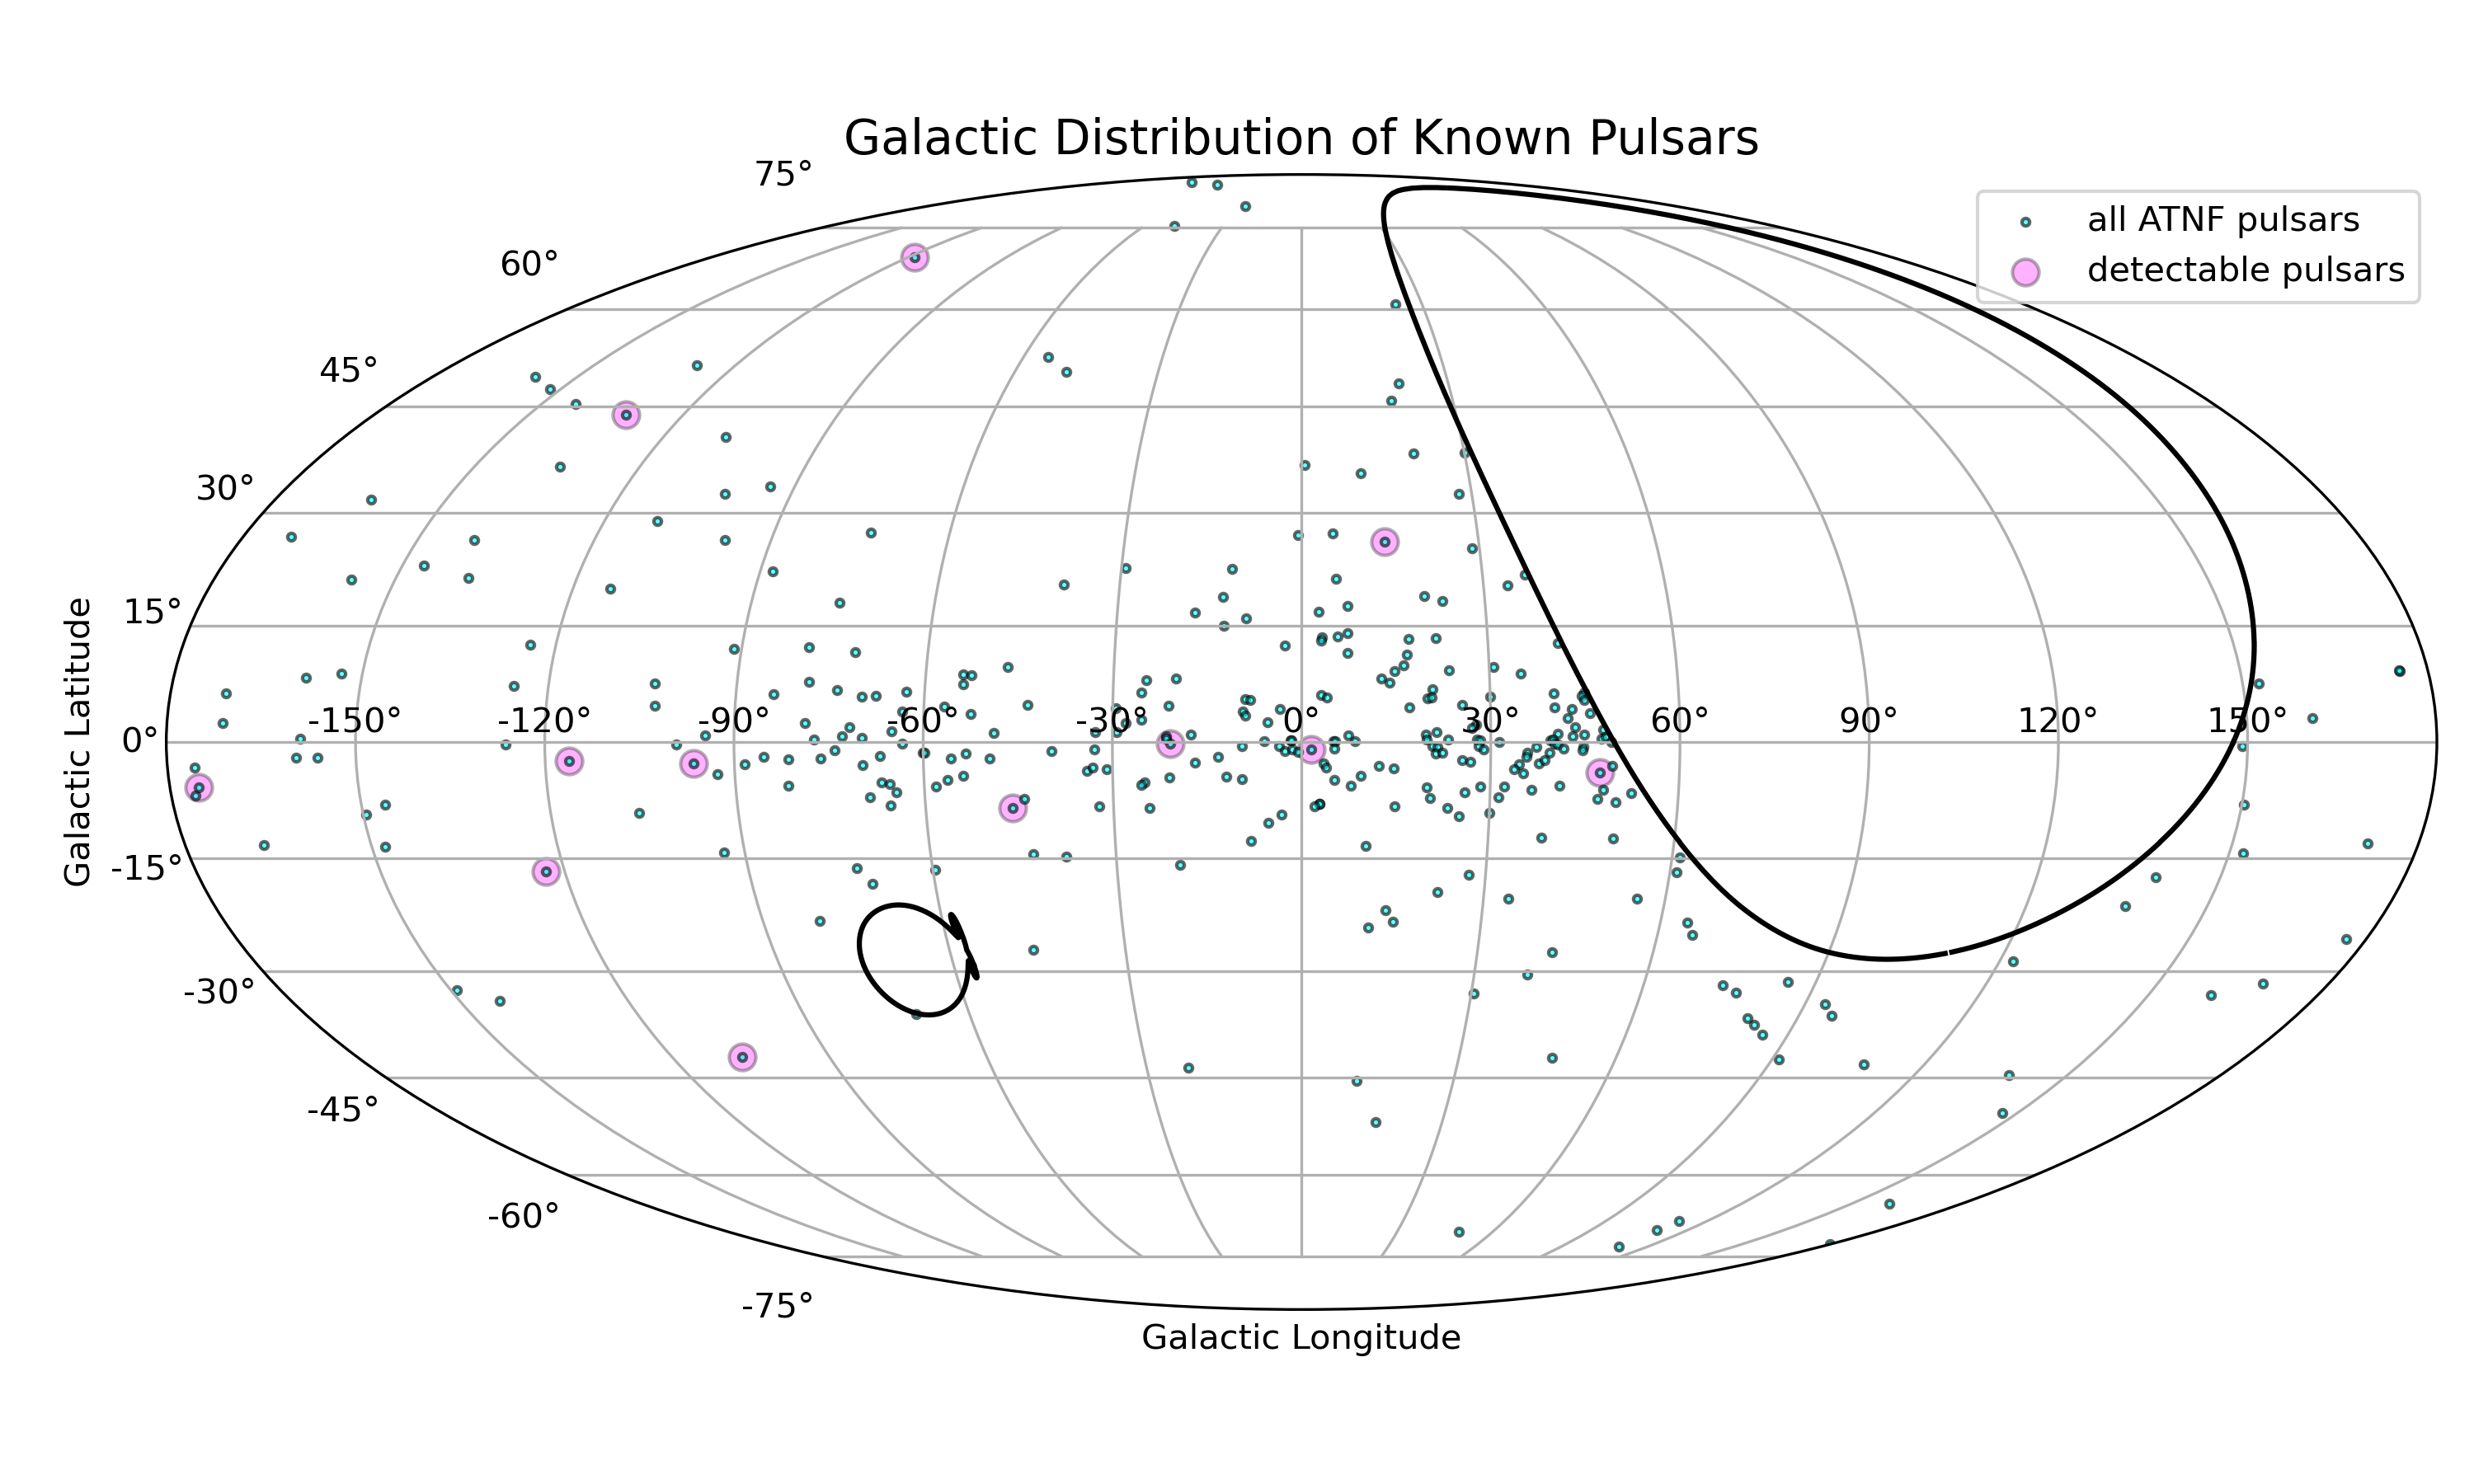
\includegraphics[width=0.8\textwidth]{figures/PulsarDectability.png}
    \caption{Distribution of pulsars detectable by LFT3 in 10 hours of observing at 400 MHz (image borrowed from \citealt{prabu2025lft3}).}
    \label{fig:pulsarDectability}
\end{figure}


\subsubsection{Fast Radio Bursts}
Fast Radio Bursts (FRBs) are intense,
%\footnote{Most FRBs have a peak flux of 0.1 Jy to a few 100's of Jy. The brightest ever seen was a Galactic FRB that emitted MJy emission},
millisecond-duration radio pulses originating from extragalactic sources. 
%Their origins remain one of the most intriguing mysteries in modern astrophysics. 
Although Galactic magnetars have been shown to exhibit similar FRB-like emission \citep{BC_2020,chime2020sgr1935}, the exact progenitors and emission mechanisms are still unknown, but the consensus is that they involve emission from neutron stars~\citep{ck21}. Some bursts are observed from stellar environments which show evidence for recent star-forming activity, e.g.~\citet{piro2021}. The stellar environments of other sources such as FRB 20200120E suggest that FRB progenitors may emit bursts long after star formation activity~\citep{kirsten2022m81} has ended, providing evidence for multiple formation channels.

The Canadian Hydrogen Intensity Mapping Experiment (CHIME) telescope is currently the world leader for detecting new Fast Radio Bursts with its 200\,deg$^{2}$ field-of-view and observing frequency of 400--800\,MHz, and outrigger stations for burst localization~\citep{leung2021synoptic,lanman2024kko}. 

A low-frequency lunar telescope, capable of high-time-resolution observations, could greatly advance our understanding of fast radio bursts, as their low-frequency emission properties are a clear factor in understanding the source populations. LFT3, supplemented by wide field-of-view ground stations on Earth could be used to co-observe to enable microarcsecond localization of the brightest FRBs, something which would be of unprecedented scientific value (see e.g. \citealt{nimmo_burst_2023}). 
%Currently, the Canadian Hydrogen Intensity Mapping Experiment (400--800\,MHz; \cite{CHIME_RepeatingFRB}), with some more recent contributions from the Five-hundred-meter Aperture Spherical Telescope collaboration \citep[1.00--1.45\,GHz;][]{ZX_2023} and the DSA-110 \citep{LC_2023,sharma2024preferential}. 
Observing beyond RFI and the ionopshere, and taking advantage of the clean FM band, may provide a key understanding to unlock the true nature and originating source of emission.

Low-frequency observations of FRBs are crucial for understanding their propagation through the intergalactic medium, potentially unveiling the distribution of baryonic matter and offering clues about the emission mechanism and source plasma environments. LOFAR observations of FRB 20180916 have revealed potential evidence for the interaction between a neutron star and its binary companion by observing bursts to 100 MHz~\citep{pleunis2021lofar}.

\textbf{System Implications:} Detection of FRBs at low frequencies requires high time resolution ($\leq$1\,ms) and sufficient spectral resolution ($\sim$0.1--0.5\,MHz) to resolve dispersion sweeps and intrinsic burst structures. While most FRBs peak between 400--800\,MHz, several have been observed down to $\sim$100\,MHz, with flux densities ranging from $\sim$0.1 to hundreds of Jy~\citep{pleunis2021lofar}. The dual polarization capability and dynamic spectra in Stokes parameters I and V will support burst characterization. Observations in the sub-100\,MHz range, inaccessible from Earth, may uncover a suppressed or scattered FRB population and place limits on free-free absorption and propagation effects. LFT3's large field of view and ability to co-observe with ground-based arrays would also enhance the chance of real-time detection and subarcsecond localization. In order to demonstrate LFT3's capacity to detect FRB-like signals, in Figure \ref{fig:FRBdetectability} we show the number of CHIME FRBs detectable by LFT3. 

% \textbf{CL: It is possible to estimate the FRB rate from CHIME, which detects about 1000 bursts per full year of observation in the same frequency range over a 200 deg$^2$ FoV with a coherent SEFD of 50 Jy. Assuming a Euclidean population of sources, in the coherent FoV of LFT3 of $\sim 4000$ deg$^2$ at the bottom of the mid-band, $\sim 0.88-2.5$ bursts could be detected per year of observation.}

\begin{figure}[h]
    \centering
    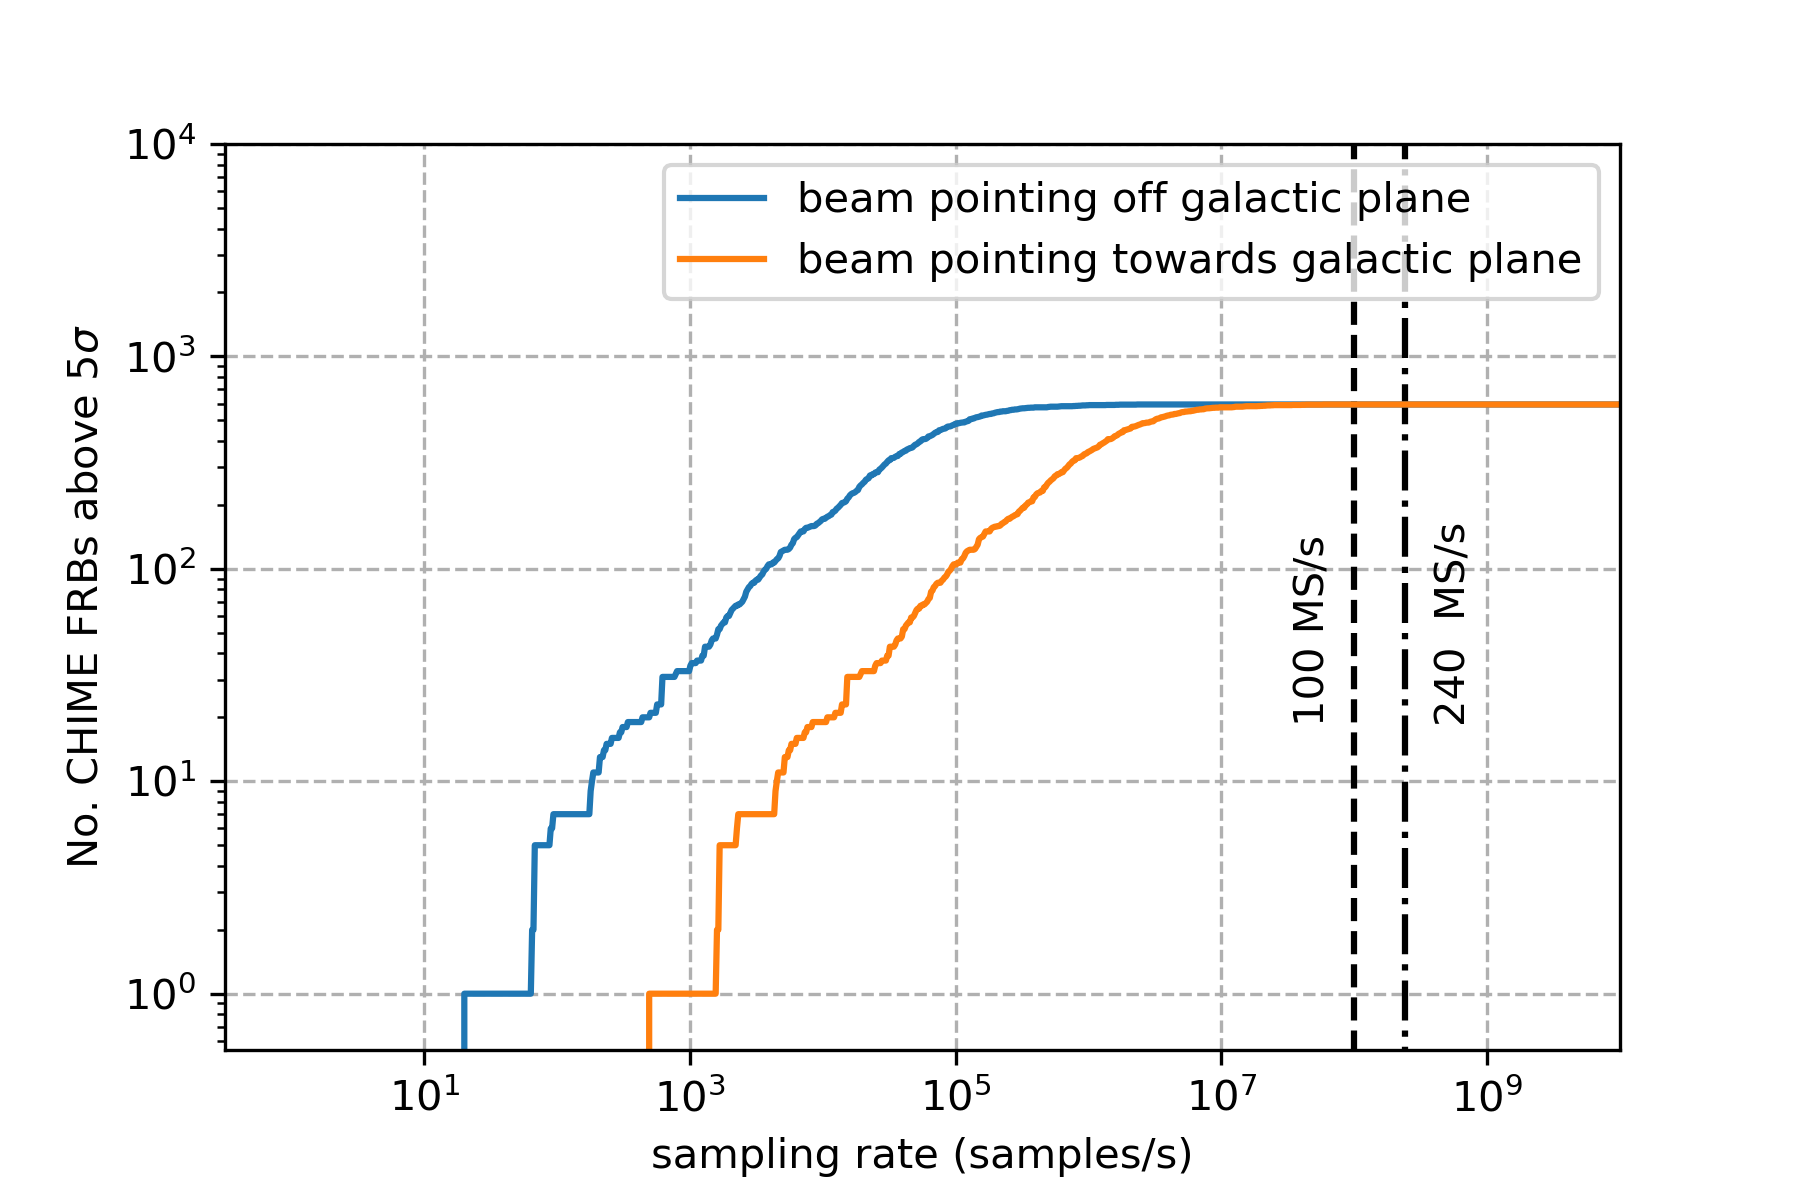
\includegraphics[width=0.8\textwidth]{figures/FRBdetections.png}
    \caption{Number of CHIME FRBs detectable by LFT3, as function of sampling rate. We show two different lines for Galactic and off Galactic pointings (image borrowed from \citealt{prabu2025lft3}).  Note that CHIME performed these detections by observing the sky for orders of magnitude more duration than the life of the proposed LFT3 mission. The objective of the plot is to show that LFT3 is well suited to perform serendipitous FRB discoveries (by showing that most of CHIME FRBs are detectable by LFT3), the offchance that such an event where to happen within the FOV of the instrument during its mission life.}
    \label{fig:FRBdetectability}
\end{figure}



\subsubsection{Long-Period Transients}
Galactic long-period radio transients represent a burgeoning new subclass of transients. Distinguished by their exceptionally long periods, minute-long pulse duration, and low-frequency emission. The prototypical example is GLEAM-X J162759.5-523504.3 \citep{hurley_walker_radio_2022}. This object exhibits a period of 18.18 minutes and a pulse duration of $\sim 1$ minute at 100--200~MHz. The measured DM for this source was $\sim57~\text{pc cm}^{-3}$ indicating a Galactic origin. The distribution of pulses seen from this source are orders of magnitude larger (30--60~s) than that of FRBs and have fluxes of 5--40~Jy. This makes their discovery and cataloging one of the most feasible and impactful science goals of LFT3 (see Fig. \ref{fig:transient_space}). The emission is also highly linearly polarized (90\%) with a spectral index of $\sim 1.2$, suggesting a strongly magnetized engine (\citealt{Men_2025}).
%It was initially thought that magnetars may be a plausible source for these transients. However, the general absence of multiwavelength emission from these sources contradicts many models (references),  leaving the discussion of the origin of these transients still on the table. 
Subsequent surveys have revealed more of these objects with periods ranging from minutes to hours (\citealt{HW_2024}). In particular, they show low dispersion measures ($\lesssim$ few $10^2~\text{pc cm}^{-3}$) which make them relatively easy to distinguish from when observing at low frequencies. They sources are not exceedingly rare and harbor many open questions yet to be fully explored.

LFT3 presents a unique opportunity to advance this field while still in its infancy. As previously discussed, having broadband observations of these sources in an RFI pristine environment will give further insight into these objects. Such observations could reveal whether these ultralong-period objects exhibit even longer-wavelength emission, test how their spectra evolve, and potentially catch new transients with ultralow dispersion measures in the local Galaxy at these ultra-low frequencies. 

\textbf{System Implications:} Long-period transients, with pulse durations of 30--60\,s and peak flux densities ranging from 5--40\,Jy at 100--200\,MHz~\citep{hurley_walker_radio_2022}, are well within the detection capabilities of LFT3. Observations should include dual-polarization data to capture the high linear polarization fraction ($\sim$ 90\%), with a spectral resolution of 0.1---- 0.5\,MHz and a time resolution on the order of 1--5\,s to resolve burst profiles while preserving sensitivity to slow periodicity. The observed low dispersion measures ($\lesssim$200\,pc\,cm$^{-3}$) reduce computational demands for de-dispersion, enabling efficient real-time searches. 

% THIS TABLE WILL BE REPLACED BY A SERIES OF PLOTS FOR THE DIFFERENT SECTIONS
%\begin{deluxetable*}{ccccccc}
%    \tablecaption{Minimum Detectable Flux Densities ($S_{\text{min}}$) Grouped by pulse width.\label{tab:smin} for 48 element Vivaldi phased array feed.}
%    \tablehead{
%    \colhead{Pulse Width} &
%    \colhead{Frequency} &
%    \colhead{Wavelength} &
%    \colhead{$A_{\text{eff}}$} &
%    \colhead{Gain} &
%    \colhead{SEFD} &
%    \colhead{$S_{\text{min}}$} \\
%    \colhead{(ms)} &
%    \colhead{(MHz)} &
%    \colhead{(m)} &
%    \colhead{(m$^2$)} &
%    \colhead{($10^{-3}$\,K/Jy)} &
%    \colhead{(kJy)} &
%    \colhead{(Jy)}
%    }
%    \startdata
%    \textbf{0.1}   & 250 & 1.2 & 17.1 & 6.2 & 16.2  & 572.5 \\
%                   & 500 & 0.6 & 4.3  & 1.5 & 64.8  & 2290.2 \\
%                   & 750 & 0.4 & 1.9  & 0.7 & 145.7 & 5152.9 \\
%    \hline
%    \textbf{1}     & 250 & 1.2 & 17.1 & 6.2 & 16.2  & 181.1 \\
%                   & 500 & 0.6 & 4.3  & 1.5 & 64.8  & 724.2 \\
%                   & 750 & 0.4 & 1.9  & 0.7 & 145.7 & 1629.5 \\
%    \hline
%    \textbf{10}    & 250 & 1.2 & 17.1 & 6.2 & 16.2  & 57.3 \\
%                   & 500 & 0.6 & 4.3  & 1.5 & 64.8  & 229.0 \\
%                   & 750 & 0.4 & 1.9  & 0.7 & 145.7 & 515.3 \\
%    \hline
%    \textbf{100}   & 250 & 1.2 & 17.1 & 6.2 & 16.2  & 18.1 \\
%                   & 500 & 0.6 & 4.3  & 1.5 & 64.8  & 72.4 \\
%                   & 750 & 0.4 & 1.9  & 0.7 & 145.7 & 162.9 \\
%    \hline
%    \textbf{1000}  & 250 & 1.2 & 17.1 & 6.2 & 16.2  & 5.7 \\
%                   & 500 & 0.6 & 4.3  & 1.5 & 64.8  & 22.9 \\
%                   & 750 & 0.4 & 1.9  & 0.7 & 145.7 & 51.5 \\
%    \hline
%    \textbf{10000} & 250 & 1.2 & 17.1 & 6.2 & 16.2  & 1.8 \\
%                   & 500 & 0.6 & 4.3  & 1.5 & 64.8  & 7.2 \\
%                   & 750 & 0.4 & 1.9  & 0.7 & 145.7 & 16.3 \\
%    \enddata
%    \tablecomments{
%    Minimum detectable flux densities are calculated assuming a system temperature of 100\,K, a bandwidth of 100\,MHz, and a signal-to-noise ratio of 5$\sigma$.
%    }
%\end{deluxetable*}
    
    
    
    

\subsection{Spectral Lines}
Radio frequency interference has a significant impact when studying Galactic and extragalactic chemistry, especially in the frequency range around 1\,GHz (e.g. \citealt{Liang_2023}). This is due to an increasingly cluttered frequency band of intense signals from anthropogenic RFI, often leaking into protected radio astronomy bands. This impacts our ability to study the chemistry, kinematics, and age of astronomical objects through the spectral properties of atoms and molecules. Therefore, we must look to more creative ways of observing the Galaxy to study the dynamical motions and slow changes that are happening over the life-spans of stars and galaxies, which are critical aspects for understanding their evolution.

\subsubsection{Extra-galactic HI}
Hydrogen is the most prominent element in the Universe and the neutral hydrogen (H{\sc I}) line at 21\,cm (1.420\,GHz) is one of the most prominent diagnostic lines used in radio astronomy. From testing models of the early Universe (i.e. \citealt{Meiksin_2022}) to tracing the spiral arms of our Galaxy \citep{HI4PI}, H{\sc I} is an important line for understanding motions and dynamics (i.e. \citealt{Pingel_2022}). However, on Earth, even though the spectral region around the 1.42\,GHz emission is protected and reserved for radio astronomy, the spectral region around the line is heavily polluted with RFI and LFT3 could augment ground-based surveys (i.e. \citealt{Bhat_2005,Rhee_2023}. This makes it challenging to study galaxies within our local Universe and beyond.

The neutral hydrogen line, observed at 1.42 GHz within our Galaxy, shifts to lower frequencies as $(1+z)^{-1}$ as a function of the distance to the galaxy at redshift $z$ due to cosmic expansion. For galaxies at cosmological distances, there will be many galaxies in each beam, and we measure their aggregate emission as a function of redshift. This is known as the intensity mapping technique. Although there were several proof-of-principle measurements on the ground \citep{Paul_2023}, this remains a challenging technique due to foregrounds that are many orders of magnitude brighter. The unique gain stability and RFI cleanliness offered by the lunar farside might offer a novel handle on controlling the foreground emission.  

\textbf{System Implications:} For this work, the data product would need to be a time-averaged power spectrum of beamformed targets or an incoherent sum. A spectral resolution of 100 kHz would be sufficient due to Doppler broadening of the 21\,cm signal. % However, if the focus is on more distant galaxies then 1~kHz frequency resolution would be preferred. 

\subsubsection{Radio Recombination Lines}
The diffuse cold neutral medium (CNM; T$_{s}$ $<$ 100\,K) is an important component of the interstellar medium (ISM). To date, this gas has been studied primarily using the 21 cm H{\sc I} line in absorption \citep{Dickey_1990}. A powerful and complementary probe of the conditions in the neutral ISM is provided by the cold radio recombination lines (CRRLs) that arise in this ionized gas. The low ionization potential of carbon atoms (11.4 eV) allows them to be ionized by far-UV radiation, leading to the subsequent production of CRRLs when free electrons recombine with carbon ions. CRRLs at low radio frequencies ($<$ 1.5 GHz) have been detected in the Galactic plane in both emission and absorption with a number of telescopes (e.g. \citealt{Kantharia_2001,Salas_2019,GDIGS}). 

At large n-bound states, observed at frequencies less than 100 MHz, the relative populations of atomic energy levels are mainly controlled by collisional processes \citep{Tremblay_2018}. These collisions drive the level populations toward thermal equilibrium with the cold gas environment (typically $< 100$ K), resulting in the detection of these lines in absorption against strong background continuum sources. The population becomes inverted at lower n-bound states at frequencies greater than 200\,MHz, resulting in emission lines being detected \citep{Gordon-RRL}. In the range of 100 to 200\,MHz, the conversion will take place at a frequency and intensity dependent on the temperature and density of the gas within the cloud. This means that the conversion will shift toward higher frequencies as the gas density increases. This makes CRRLs excellent pressure and temperature probes of the ionized gas regions of the ISM \citep{Salas_2019}.

The ionosphere negatively impacts scientific measurements as a wavelength squared dependence, thus having a greater impact on lower-frequency observations. Observing low-frequency ($<$ 500\,MHz) CRRLs is critical to understanding the temperatures and conditions of ionized gas fronts in cold gas \citep{Salas_2018}. Placing a telescope far above the ionosphere would prevent ionospheric data artifacts and extrinsic spectral line broadening, which could erroneously change the measured conditions.

\textbf{System Implications:} The CRRLs will change width depending on the frequency of detection and the conditions of the environment. However, a resolution of 0.5\,kHz would be sufficient to study the lines across proposed frequency bands. Additionally, an initial time resolution of 8-10 seconds is sufficient, with the option to average data over longer periods to increase sensitivity so long as the source remains within the field-of-view. We do this with nonmoving dipoles with ground-based telescopes by either employing fringe tracking or by doing short time recordings, correcting for the source position, and then time-averaging the data. If the dipoles were treated as independent entities, correlated visibilities would allow for a low-resolution map of the regions where the signals are detected. Additionally, beamforming can be used in two approaches: coherent beamforming, which maximizes sensitivity for known source positions, or incoherent beamforming, which sacrifices some sensitivity for a wider field of view and is more robust when detecting strong spectral lines. Overall, a spatial resolution of one degree in the sky would allow for follow-up by ground-based telescopes, where more detail is required. The preferred output is a time-averaged power spectrum or a spectrum converted to intensity in Jy. Either way, a calibration of the flux density values will be needed.

\subsubsection{Blind search for novel spectral features}

There are several mechanisms with varying levels of speculation that could produce novel spectral features in the data. Leading among them would be interactions in the dark-matter sector \cite{2025ApJ...984L..24K}.  Many of such lines could be in regions of the spectrum that are heavily impacted by the RFI or the ionosphere and could have escaped detection so far. In most models these correlate with galaxies, but in some models, such as Dark Photon Dark Matter \citep{2025PhRvL.134q1001A} they appear to correlated with the Sun.  LFT3 is perfectly positioned to perform a blind search for weak new spectral features across all observed radio bands that correlate with either the Galaxy or the Sun. 

Another region of study for novel spectral lines is low-frequency masers. Spectral lines below 1\,GHz from certain molecules indicate non-thermal emission \citep{Tremblay_2017}. However, as demonstrated for Nitric Oxide by \cite{Tremblay_2020_NO}, the prominent transitions at 107\,MHz are significantly impacted by RFI as it resides in the FM radio band. This is true for many of the molecules of interest that have been studied by ground-based radio telescopes (\citealt{Jacob_2024}).

Therefore, a telescope on the moon could provide a significant benefit in understanding the gas evolution, kinematics, and chemistry of astrophysical environments, away from the influence of Earth-based RFI.

\subsubsection{Cosmology}
Radio observations of red-shifted atomic hydrogen have the potential to uniquely inform our knowledge of the early Universe, from the so-called Cosmic Dark Ages over 13 billion years ago, to the formation of the first stars and black holes that reionized the Universe in its last cosmic-wide change \citep{Fialkov_2024}. This is because neutral hydrogen was the dominant form of baryonic matter during this period and can be detected on the basis of its 21 cm spectral line (rest frequency 1420 MHz). Of particular interest is the rise of the astrophysical structure in the cosmic fabric beginning about 13 billion years ago.  Since the relevant signal emanates from a distance of 13 giga-lightyears (Gly), it is exceedingly faint, requiring extreme sensitivity and radio-quiet conditions.  Since the signal of interest is also global, a single antenna is technically sufficient.  Figure \ref{fig:cosmo_h} shows a cartoon of cosmic evolution as a function of age (top) and redshift (bottom) and maps that to the observed frequency of redshifted hydrogen (yellow line).

Due to strong emission from our Galaxy at the relevant frequencies, the sky is extremely bright, with brightness temperatures ranging from about 100 K to $10^6$K depending on frequency and location, while the signal of interest is very faint (in the milliKelvin range), hence the difficulty in making the measurement.  Figure \ref{fig:global_T_bw} shows one model of the cosmological signal strength (taken from \citealt{Fialkov_2024}) across frequencies (and hence cosmic time).  Note that the observable is the difference between the hydrogen spin temperature and the CMB temperature and may be positive or negative.  Making this measurement requires extremely precise knowledge of the smooth shape of the measured spectrum and removing this as a baseline.  Low-level unaccounted for RFI adds uncertainty to any measurement. Precise measurements from the RFI quiet lunar farside will be invaluable in understanding that effect.

Note that LuSEE-Night, which should launch early 2026, is similarly focussed on making measurements relevant to the global signal, with all of its inherent difficulty.  LFT3 will work in collaboration with LuSEE-Night to help inform these measurements.  Both missions will fly the same HF antenna, although by necessity the physical arrangements will differ.  Ideally, both would operate at the same time; however, this would require LuSEE-Night to remain operating for several years.  There is the possibility of using the same calibration orbiter, which is a payload delivered by LuSEE-Night.  One of the primary difficulties in this measurement is the affect of the lunar regolith on the received signal, and having two nearly identical systems in close proximity may be able to uniquely inform this issue.

\begin{figure}
    \centering
    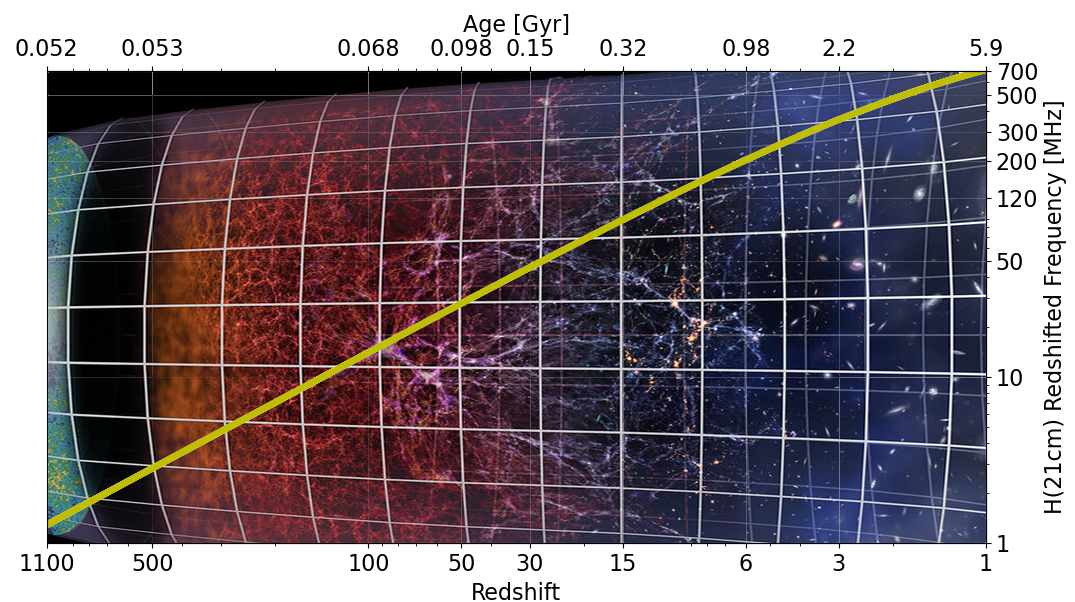
\includegraphics[width=0.8\textwidth]{figures/zage_lft3_python.png}
    \caption{Cosmic evolution and observability by red-shifted hydrogen.  The underlying cartoon (credit: ESO/M. Kornmesser) shows a depiction of cosmic evolution from the era of the cosmic microwave background (on the left) to the near-modern era.  The top horizontal scale shows time after the Big Bang in Gyr and the bottom the associated red-shift.  The yellow line and vertical axis indicate the observable frequency at that age.  LFT3 has receivers across this entire range.}
    \label{fig:cosmo_h}
\end{figure}

Although it is highly unlikely that LFT3 would have sensitivity to detect either the Dark Ages or the Epoch of Reionization signals in the monopole, in the HF it could detect excess photons in the Rayleigh-Jeans tail of the CMB spectrum, which could again put strong limits on some dark matter models \citep{2018PhRvL.121c1103P}. In fact, there have been long-standing hints on excess emission in the radio sky at low frequencies (\cite{2018ApJ...858L...9D,2011ApJ...734....4K}) and this is something LFT3 is uniquely positioned to test. 


\textbf{System Implications:} 
The expected signal is thermal; however, that thermal profile changes with cosmic time and hence frequency, so the bandwidth and binning impact the result (see, e.g. \citealt{2017PASP..129d5001D}).  Figure \ref{fig:global_T_bw} shows the impact of using the 1 MHz and 10 MHz bands for this model and indicates that a few MHz bandwidth is desired\footnote{Using as large of a bandwidth as possible is desired, since that reduces the system noise, however it can smear spectral structure.}.  Long integrations improve the sensitivity, so FOV changes on the order of minutes are the limiting factor.
Given the noise of the Galactic plane, the Sun, and Jupiter, it is preferable to observe when they are all below the horizon.

\begin{figure}
    \centering
    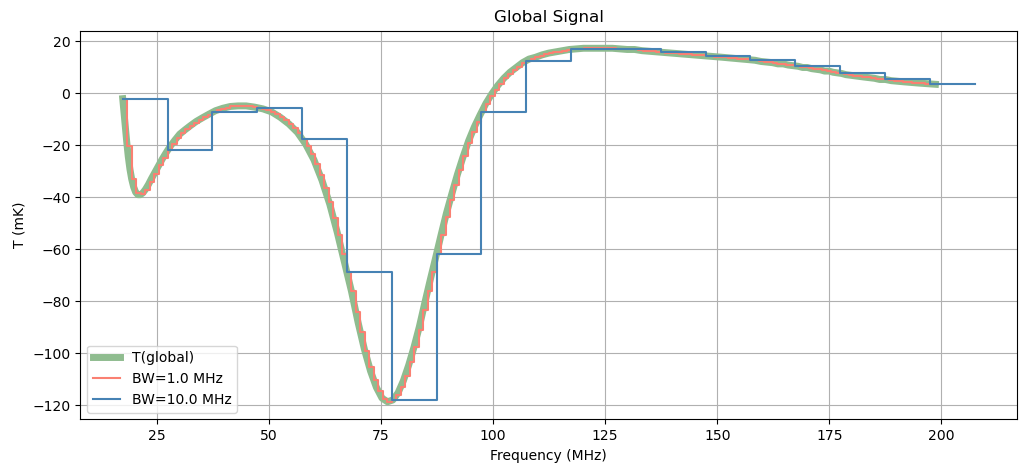
\includegraphics[width=0.8\textwidth]{figures/global_with_bw.png}
    \caption{Global signal from the early Universe (green), which is the difference between the hydrogen spin temperature and the cosmic microwave background temperature, as taken from \cite{Fialkov_2024}.  The blue line shows the effect of a 10 MHz measurement band, while the orange (nearly coincident with the green curve) shows the effect at 1 MHz.}
    \label{fig:global_T_bw}
\end{figure}

\subsection{Polarization modulation by axion-like dark matter}
There has been a renewed interest in cosmology in ultralight dark matter candidates \cite{2022SciA....8J3618C}. This framework postulates a dark matter particle with such a small mass that its de Broglie wavelength spans roughly a kiloparsec—coinciding with the scale where structure formation issues arise. This corresponds to a particle mass around $m\sim 10^{-22}$\,eV. Due to this extremely low mass, achieving the observed dark matter energy density necessitates a very high number density of ULDM particles, implying that they behave collectively as a classical bosonic field, or a Bose-Einstein condensate. To stabilize this tiny mass against radiative corrections, it is typically assumed that the ULDM field is a pseudo-Goldstone boson resulting from a broken symmetry analogous to the QCD axion, which stems from the breaking of the Peccei-Quinn symmetry. Whether connected to QCD or not, such particles tend to couple to photons through non-renormalizable interactions, similar to those of axions. Particles of this kind, known as axion-like particles (ALPs), arise naturally in many beyond-the-Standard-Model scenarios, including string theory frameworks.

Coherent field oscillations of ALPs affect the propagation of electromagnetic waves through the ULDM condensate. It has been shown \citep{2019JCAP...02..059I,2024PhRvD.110f3013A} that the polarization angle of linearly polarized light oscillates with the same period—set by the ALP mass—which remains constant across all ALP domains in the Universe. The prediction is that the polarization angle of linearly polarized radio emission oscillates in time, which can, in principle, be detected with an instrument such as LFT3.  In fact, LFT3's unique gain stability given the lunar environment and slow moon rotation allowing for long dwelling time should make it particularly sensitive to search for linearly polarizated light oscillations. 

\textbf{System Implications:} 
The expected signal is weak and the polarization angle can appear to oscillate due to the gain mismatch between two polarization state channels and the variable leakage of polarization due to thermal expansion. The system should be designed to maximize the benefit of a stable environment on the lunar farside.



\subsection{Exploration of VLBI Techniques}
Very Long Baseline Interferometry (VLBI) is a powerful technique of using a large separation between antennas to obtain incredible detail of astronomical objects. This method is often used to study galaxy evolution and variability (i.e. \citealt{Sheldahl_2025}), the precise location of sources of maser emission (i.e. \citealt{Shinnaga_2025}), and the study of proper motion (i.e. \citealt{Kumar_2025}). More recently, the Event Horizon Telescope (EHT; \citealt{Chael_2018}) has used the techniques of VLBI to study black holes at the center of galaxies to provide incredible scientific detail to the regions \citep{M87}.

By having a telescope on the moon with a wide range of frequency coverage, we could collaborate with ground-based facilities to test Earth-Moon VLBI methods. As the earth-based telescope has to contend with the ionosphere, joint measurements would not be available for most of the HF band ($<$30\,MHz). However, the other bands have significant overlap with ground-based telescopes in both the southern and northern hemispheres.  Joint experiments with multiple facilities from VHF to UHF will be explored. 

\textbf{System Implications:} To accomplish the goal, we would need to transmit time-stamped baseband data, coordinate an observation toward a shared patch of the sky, and provide precise timing clocks. We could then use a combination of conventional VLBI correlation and fridge fitting and techniques used by the EHT, which uses a more model-fitting approach to explore this technique for scientific study of the cosmos.

\subsection{Lunar Environment}
Along with advancing astronomical science, operating a telescope on the moon will also yield invaluable insights into the lunar environment and details regarding the engineering and functionality of lunar telescopes. These insights can be classified into (1) the RF environment, (2) the physical environment, and (3) the operational/engineering, as discussed below. 

\subsubsection{RF Environment and Spectral Monitoring}
Although the lunar farside should be a pristine RF environment, there is the potential of some RFI from the lunar communication orbiters that will be in place, as well as spacecraft that are at distances further than the moon.  There is also the potential of unknown actors emitting radio frequencies, as well as additional payloads being deployed during the LFT3 operational period, for example China's orbiting interferometer called ``Discovering the Sky at the Longest Wavelengths'' (DSL).  As mentioned throughout, this is a time of unique change in the operating cislunar environment, and measuring a legacy spectral baseline as well as the potential increasing emergence of RFI is a key objective of this mission.

The dynamic spectra taken over the operational period and transmitted back to Earth will provide the key record of the baseline and evolving RF spectrum and LFT3 represents the {\bf only mission} proposed to make these measurements.  In addition to the dynamic spectrum, LFT3 will catalog {\em every} measured RF event.  This will allow a unique record of the changing cislunar RF environment.

\subsubsection{Physical Environment}
The primary environmental factors of the lunar physical environment are the properties of the regolith and the extreme temperature range.  The moon does have a tenuous ionosphere due to solar ultraviolet radiation interacting with the lunar surface, but likely very limited impact for LFT3.  These factors obviously strongly affect the operational and engineering aspects below; however, the regolith is particularly an interesting object of study. Regolith is a term used to describe any loose, unconsolidated material above the bedrock of a celestial body. The lunar regolith has effectively three different science impact components for LFT3: (1) electromagnetic, (2) structural, and (3) dust.

{\em Electromagnetic.}  The electromagnetic properties of the regolith have a huge impact on the mission, particularly at the lowest frequencies and for cosmology.  Understanding the lunar surface topography, conductivity, dielectric constant, emission, and reflection of radiation is the key to understanding its impact on scientific results.  For the Cosmic Dark Ages science, this is arguably the most important component.  The EM missions as part of NASA's Commercial Lunar Payload Service (CLPS) are essentially all leveraged to understand the lunar environment and interactions with the regolith, such as ROLSES \citep{2025arXiv250309842H}, LuSEE-Night \citep{2023URSIGASSLuSEENight, 2023arXiv230110345B} and LuSEE-Lite \citep{2023AGUFM.P31B..02B}.  LFT3 would complement those efforts and will conduct coordinated experiments with LuSEE-Night, near which LFT3 will land.  Being nearby will allow studies of the same region but from a different vantage point and will provide additional information on the affects of the regolith.

{\em Structural.} LFT3 provides a unique opportunity to investigate the structure and composition of the regolith at its landing site in the farside highlands.  The Moon is globally covered in inorganic regolith (also called lunar soil) about 4-5 m thick in the highlands and 10-15 m thick in the lowlands, synonymous with the lunar maria that stretch along the near side of the Moon \citep{mckay1991lunar}. The highlands are older, more heavily cratered regions that make up the vast majority of the farside and include LFT3's landing site.  As with all lunar regolith, the highland regolith has formed over billions of years from the steady erosion of bedrock by meteorite impacts. Highland regolith, based on samples examined on the near side of the Moon, has an anorthositic composition (anorthosite is an intrusive igneous rock formed when lava forms intrusions within existing rock and crystallizes) composed primarily of silicates and metal oxides.

Characterization of the regolith at LFT3's landing site will be of significant interest to engineers and planetary scientists, especially given that only two missions, Chang'e 4 \citep{wimmer2020lnd} and Change'e 6 \citep{Ren2025ChangE6}, have successfully landed on the farside to date\footnote{Chang'e 6 returned samples of the lunar farside}. Such characterization will provide insights into the local regolith's physical properties.  Fortunately, vital information can be obtained without dedicated sensors, using the systems already on board the lander, such as its IMU (inertial measurement unit) and touchdown sensors.  For example, Firefly Aerospace's \textit{Blue Ghost} lander, the first commercial lander to have a fully successful soft lunar landing, has footpad sensors to determine the moment when its feet contact the lunar surface \citep{Firefly2025BlueGhost}.  In combination with data from the high-resolution IMU that any lander would already possess, and a detailed dynamical model of the lander itself, a relationship can be determined between the forces the lander experiences during landing and the subsidence of the regolith.  An iterative multiphysics model could predict the IMU response based on the established timeline of the landing and assumed geotechnical properties of the site's regolith (based on other landing missions), such as its angle of internal friction and cohesion.  Iterating this model until the predicted response converges with the measured response should produce an estimate of the actual properties of the regolith at the landing site.  Constraining these properties would be of high value for any future landings in similar lunar environments, as these properties themselves constrain the design of landers and any other structures to be stably placed on the lunar surface without subsiding.  Measuring the rate of the lander's temperature change throughout the lunar night, which is already required for lunar night survival, will allow estimation of the regolith's thermal conductivity, as the lander will lose heat by conduction to the lunar surface in addition to otherwise expected radiative loss.

Further low-cost sensors could greatly improve this analysis.  For example, the first \textit{Blue Ghost} mission included a set of six cameras called SCALPSS (Stereo Cameras for Lunar Plume-Surface Studies), which successfully filmed the lander's descent and touchdown from multiple angles 8 frames per second \citep{Atkinson2025NASA}. The images from these cameras are used to create digital elevation maps of the landing site via stereo photogrammetry. By observing how these maps change throughout the landing process, as the lander's exhaust plume scours the surface, researchers could estimate the total volume of regolith ejected, how the rate of ejection varies over time, and the depth of the removed layers \citep{Tyrrell2022PlumeSurface}.  These data, when analyzed together with a multiphysics model of the landing, could reveal how the properties of the regolith vary with depth near the surface.  Characterizing plume-surface interactions, as with the SCALPSS experiment, could also help quantify the hazards to surrounding infrastructure posed by landing on unprepared lunar surfaces nearby.  Even something as simple as having cameras with the lander's footpads in view could reveal their penetration depth into the regolith after landing, allowing the regolith's bearing capacity to be calculated.  

Any of these low-cost measurements and analyses will be valuable for planning future missions and improving the quality of lunar simulations.


{\em Dust.} The top surface of the moon comprises a very fine dust with 20\% of particles by weight having a diameter below 20 \textmu m \citep{ZANON2023627}.  Lunar dust is very abrasive and becomes electrostatically charged as a result of interactions with solar wind and UV radiation.  The act of landing on the moon generates copious amounts of dust that can settle on the hardware of the lander and affect performance and operations. Although electrostatically charged abrasive dust has proven destructive to mechanical joints and pressure seals, it has been less of a problem for RF hardware and antennas.  The Chang'e 4 lander has been operational since landing on the lunar farside in 2019, with no negative effects from dust noted regarding operation of its X-band antenna, lunar penetrating radar (which has channels at 60 and 500 MHz), or low-frequency radio spectrometer (which measures in the 0.1-40 MHz range) \citep{JIA2018207}.

Fortunately, proactive measures can be taken to avoid leaving the impacts of dust adherence to chance.  Voyager Space successfully tested a passive "clear dust repellant coating" aboard \textit{Blue Ghost} Mission 1, a CLPS mission, which landed on February 2, 2025 \citep{voyager2025dustcoating}.  This mission also tested NASA's electrodynamic dust shield, a low-mass system that draws 2-4 W of power to remove dust particles with electric fields using transparent indium tin oxide electrodes, which allows it to remove dust from optical sensors and camera lenses in addition to other components \citep{buhler2020current}.  The dust shield has demonstrated 98\% dust removal during laboratory testing, with improved performance under lunar analogue UV exposure \citep{WANG20246194} and the results of lunar systems are still pending.  Various passively dust-tolerant mechanisms, including seals and bearings, are also being developed \citep{fritz2024dustroadmap}.

The dust mitigation measures ultimately employed by LFT3 will help demonstrate protection of sensitive RF equipment in the lunar environment, with qualitative data on the extent and effects of dust adherence being gathered with optical imaging of the lander's instruments and RF measurements.

\subsubsection{Operational and Engineering Impact}

LFT3 will gather baseline RF spectra for the lunar farside environment, which will benefit any future farside missions that take RF measurements.  The data handling procedures established to store and transmit LFT3's measured data to Earth will similarly be useful for any future farside missions, none of which can directly transmit data to Earth.  As with the CLPS missions, LFT3 will help establish the relevant electromagnetic impacts of regolith on RF instruments, with special attention to impacts on high sensitivity, low frequency radio astronomy.

Data gathered by LFT3's IMU and surface contact sensors will allow for the estimation of the geotechnical properties of the local regolith, such as its cohesion, angle of internal friction, and bearing capacity.  Additional low-cost cameras could stereoscopically film the descent of the lander, revealing interactions between its exhaust plume and the regolith at the surface, providing information to strengthen the analyses of the regolith's properties.  Even without dedicated sensors, vital information about the regolith can be gathered for use in future lunar surface missions.

LFT3 may include a payload to assess the performance of potential lunar construction materials.  A promising candidate is the biopolymer-bound soil composite (BSC), a material comparable to concrete that binds to lunar regolith using a small fraction of a biopolymer binding agent \citep{jrm.2020.09844}. A system is envisioned to image a set of BSC samples (made with regolith simulant) and control samples (made of conventional concrete) with a pair of stereoscopic cameras.  Images taken over time will show the extent of cracking or spalling due to environmental exposure.  Miniature load cells for each sample would allow for measurement of stress due to thermal expansion and contraction, allowing for calculation of their elastic modulus and any changes to their elastic behavior over time.  Embedded strain gauges and thermocouples within the samples would provide additional complementary data.

The dust mitigation techniques employed by LFT3 will be relevant for future lunar surface missions, regardless of their specific purpose.  Alongside the CLPS missions and other future surface missions, LFT3 will play an important role in helping engineers converge on a set of practical solutions to avoid the negative effects of lunar dust adherence.

Furthermore, techniques to survive the cold night temperatures are critical to future missions, and the techniques employed by LFT3 will further our understanding of effective mechanisms.  In addition, partners will be sought to provide additional sensors or data analyses for lunar environmental characterization.

\subsection{Science Summary}
The strength of LFT3 lies in its ability to uncover the unknown while operating in a completely unprecedented environment. As the only mission with the goal of capitalizing on this unique moment in human history, LFT3 stands at the forefront of discovery.  Table \ref{tab:scisum} provides a summary of the primary science objectives along with some of their system needs.  Additionally, the robust design is tolerant to system issues that may arise in landing or operation, within the scope of the mission.

It is important to emphasize that any observation with LFT3, regardless of resolution, will be unique and scientifically valuable.  With its high-performance design, LFT3 will leave a lasting legacy, documenting the transition of the cislunar environment, potentially discovering new phenomena, and addressing long-standing questions about known phenomena. 


%In an ideal world, all data would be taken at high resolutions for both time and frequency, it  would also be obtained for as much of the sky that can seen from the cislunar enviroment for the duration of the mission. But the capacity of communications relays the byte heavy nature of radio data and on-board computing ablities all compromises will have to be made. An example outlined in Table \ref{tab:bandparam} is the acquistion of pulsar data or similar, this data can be downsampled or directly used for any of the science cases that proceed it, only limited by the integration time (i.e. Pulsar data won't last hours, which rules out exoplanets). However a similar argument can be for the opposite case, taking solar system data can be used for science applications for pulsar science for studies of younger, slower pulsar's ($P>2~\text{s}$), this argument can be applied for most the outlined science objects especially for those where the need for high frequency and time resolution diminishes (i.e. LPTs, Flar Stars, Solar System). 

%An example is having access only to an incoherent sum. This is similar to a single-dish telescope in which there is no ability to pinpoint the exact location outside the field of view of the telescope itself. The time and frequency dynamic spectrum, combined with a catalog of the sources within the field, will still provide some indication of the type of event we are seeking to study. 

%Provided we continue with a multibeam array as indicated in Figure \ref{fig:midband_beam_maps}, then a range of frequency and time resolutions will provide interesting results. Experiments such as technosignature searches can take on a range of different characteristics and can be easily molded to fit the system limitations. On the other hand, searches for FRBs may require a rigid approach to detect them and their analogs. When studying the solar system, we have little experience studying our planetary neighbors at the lowest radio frequencies, but studying lightning storms and other dynamic phenomena can benefit from the highest time resolution.  

%In general, no matter what the final system design allows, wonderful new discoveries will be made.

%TO EDIT TABLE GO TO https://docs.google.com/spreadsheets/d/1clqERhDnDB9SL_8catnJ7HusDK8cGh2FWItGwrJYpmc/edit?gid=1969441792#gid=1969441792
%CONVERT AND CUT-PASTE BACK IN
\begin{table}
\centering
\caption{System requirements for each mission objective.
Band characteristics are defined in Table \ref{tab:bandparam}. Science category 1 is Lunar-Exclusive Science, category 2 is Lunar-Augmented Science, and category 3 is Proof-of-Concept Science (see Figure \ref{fig:sciencegoals}). }
\begin{tabular}{|l|l|l|l|l|l|l|}\hline
\label{tab:scisum}
\textbf{Mission Objective} & \textbf{Receiver Band} & \textbf{Freq. Res.} & \textbf{Time Res.} & \textbf{Objects of interest} & \textbf{Stokes} & \textbf{Category} \\\hline
Technosignatures & HF/VHF/UHF & 10Hz & 1sec & catalog/blind survey & I, Q, U, V & 1,2 \\\hline
Pulsar & HF/VHF/UHF & 0.5MHz & 1ms & catalog/blind survey & I & 2,3 \\\hline
FRB Analogs & HF/VHF/UHF & 0.5MHz & 10ms & catalog/blind survey & I & 1,2 \\\hline
Flare Stars & HF/VHF & 0.5MHz & 1sec & Gaia Stars & I, V & 2 \\\hline
 & UHF & N/A & N/A & N/A & I & 3 \\\hline
Exoplanets & HF & 10MHz & hours & Nearby exoplanets & I,V & 1 \\\hline
Solar System & HF/VHF & 100 kHz & 1s & All SS Planets & I,V & 2 \\\hline
 & UHF & 1 MHz & minutes &  & I & 3 \\\hline
Studies of the Sun & HF/VHF & 0.5MHz & 1--2ms & Sun & I,V & 3 \\\hline
 & VHF & 0.5MHz & 1--2ms & Sun & I & 3 \\\hline
HI Studies & HF & N/A & N/A & N/A & I & 3 \\\hline
 & VHF/UHF & 1kHz & 5--8sec & Radio Galaxies & I & 3 \\\hline
RRL & HF & N/A & N/A & N/A & I & 2 \\\hline
 & VHF/UHF & 0.5kHz & 5--8sec & SNR, HMS$^{1}$ & I & 3 \\\hline
Cosmology & HF/VHF & 1 MHz & minutes & Non-Galactic Plane & I & 2 \\\hline
VLBI & HF/VHF/UHF &  &  &  & BB & 1 \\\hline
Lunar studies & HF/VHF/UHF & 1 kHz & 1s & Moon & I & 1 \\\hline
\end{tabular}
$^{1}$HMS=High mass star formation regions
\end{table}


%\subsubsection{Science Verification}

% Whenever a new instrument or telescope is brought online, a verification that the sytem is doing what you expect is necessary. Observational radio astronomy has been going on since World War II, creating a vast catalogue of sources and their behaviour. Therefore, we can use a combination of our knowledge of such sources and simultaneous observations with other telescopes to verify the system. 

%PLOTS That could be useful 
% Frequency/Wavelength against Flux Density of Transients -> parameter space plot 
% Variation of Tsys (basically mapping galactic forground) as a function of Lunar Latitude 
% Senstivity as function of integration time 
% Galactic latitude on the x axis, sensitivity on the y, carious longitudes overlapped. 
% Galactic projection plot for areas/exoplanets of intrest, i.e. benchmarking well known targets. 
% Also worth running some numbers to see how much time A team targets are in primary 